\chapter{Testes e Resultados} \label{chap:testsResults}
	\section{Procedimento 01}
	\label{chap:testsResults:sec:Experimento01}
	Os testes, e correspondentes resultados, para o procedimento 01 descrito no Capítulo anterior encontram-se nesta seção. Conforme explicado naquela oportunidade, este procedimento visa, com base na Engenharia Paraconsistente, encontrar qual filtro \textit{wavelet} proporciona, em conjunto com a escala Bark ou Mel, a menor distância do ponto $(G_1,G_2)$ até o vértice $(1,0)$ do plano paraconsistente. 

	\par Particularmente, na Figura \ref{fig:paraconsistentfull}, que combina os resultados dos filtros com as escalas, quanto menor o comprimento horizontal das barras na cor azul, melhor a separabilidade entre as classes. Como se pode constatar, das combinações testadas, \textbf{Haar + Bark} proporcionou a menor distância. Complementarmente, as Tabelas \ref{tab:distParacomFrom10Bark_1}, \ref{tab:distParacomFrom10Bark_2}, \ref{tab:distParacomFrom10Mel_1} e \ref{tab:distParacomFrom10Mel_2} contém os valores específicos visualizados graficamente naquela Figura.
	
	\par A combinação \textbf{\textit{wavelet} + Bark} apresentou, consistentemente, \textbf{melhor} viabilidade do que as respectivas combinações \textbf{\textit{wavelet + Mel}}.
	
	\begin{figure}[h]
		\centering
		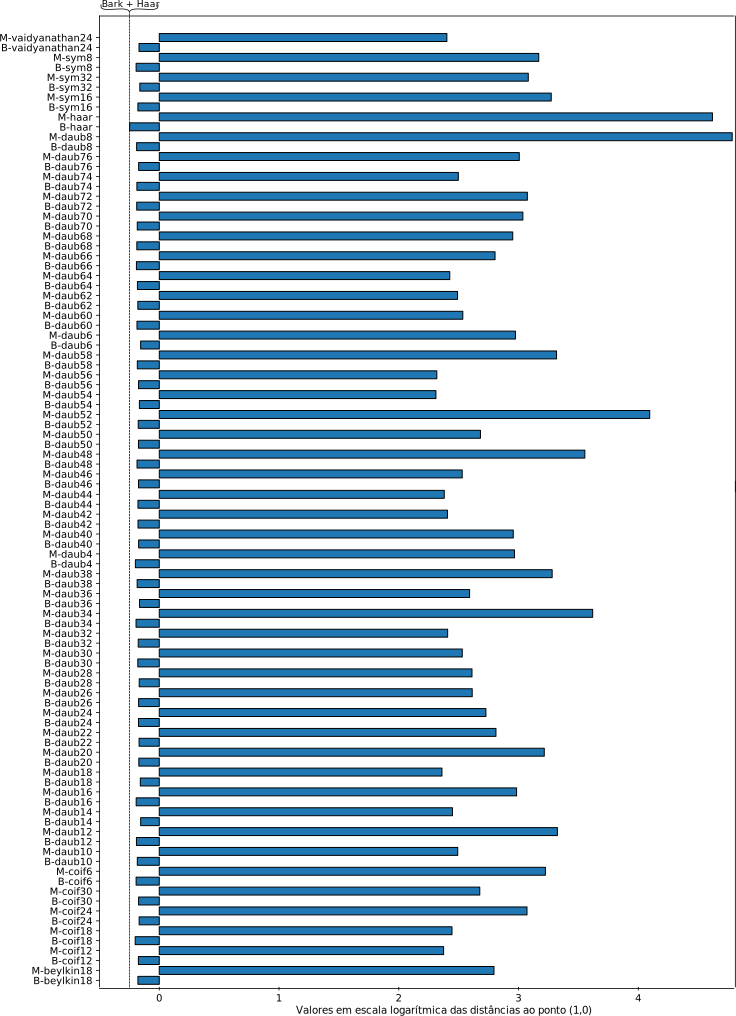
\includegraphics[width=0.99\linewidth]{images/results/paraconsistentPlane/ParaconsistentFull}
		\caption{Gráfico completo da distância ao ponto (1,0) no plano paraconsistente.}
		\label{fig:paraconsistentfull}
	\end{figure}

	\begin{center}
	\newcommand{\mc}[3]{\multicolumn{#1}{#2}{#3}}
	\definecolor{tcB}{rgb}{0.447059,0.74902,0.266667}
	\definecolor{tcA}{rgb}{0.65098,0.65098,0.65098}
	\definecolor{tcC}{rgb}{1,0.94902,0}
	
	\begin{longtable}{|p{0.25\linewidth}|p{0.25\linewidth}|p{0.25\linewidth}|p{0.25\linewidth}|p{0.25\linewidth}|}

		% Columns headers
		\hline
		\mc{1}{|>{\columncolor{tcA}}c|}{Mel/Bark}&\mc{1}{|>{\columncolor{tcA}}c|}{Wavelet}&\mc{1}{|>{\columncolor{tcA}}c|}{G1}&\mc{1}{|>{\columncolor{tcA}}c|}{G2}&\mc{1}{|>{\columncolor{tcA}}c|}{Distance to (1,0)}\\\hline
		\endfirsthead
		
		\mc{2}{c}{{\tablename\ \thetable -- continued from previous page}} \\\hline
		% Columns headers
		\mc{1}{|>{\columncolor{tcA}}c|}{Mel/Bark}&\mc{1}{|>{\columncolor{tcA}}c|}{Wavelet}&\mc{1}{|>{\columncolor{tcA}}c|}{G1}&\mc{1}{|>{\columncolor{tcA}}c|}{G2}&\mc{1}{|>{\columncolor{tcA}}c|}{Distance to (1,0)}\\\hline
		\endhead
		
		\hline \mc{2}{c}{{Continues on next page}} \\
		\endfoot
		\endlastfoot

		\mc{1}{|>{\columncolor{tcB}}c|}{MEL}&\mc{1}{|>{\columncolor{tcB}}c|}{daub68}&\mc{1}{|>{\columncolor{tcB}}c|}{-0.81987033518}&\mc{1}{|>{\columncolor{tcB}}c|}{0.16859973133}&\mc{1}{|>{\columncolor{tcB}}c|}{1.8276635101}\\\hline
		\mc{1}{|>{\columncolor{tcC}}c|}{MEL}&\mc{1}{|>{\columncolor{tcC}}c|}{daub66}&\mc{1}{|>{\columncolor{tcC}}c|}{-0.82275683686}&\mc{1}{|>{\columncolor{tcC}}c|}{0.17347376181}&\mc{1}{|>{\columncolor{tcC}}c|}{1.8309930727}\\\hline
		\mc{1}{|>{\columncolor{tcC}}c|}{MEL}&\mc{1}{|>{\columncolor{tcC}}c|}{daub46}&\mc{1}{|>{\columncolor{tcC}}c|}{-0.82442762582}&\mc{1}{|>{\columncolor{tcC}}c|}{0.1684770305}&\mc{1}{|>{\columncolor{tcC}}c|}{1.8321901298}\\\hline
		\mc{1}{|>{\columncolor{tcC}}c|}{MEL}&\mc{1}{|>{\columncolor{tcC}}c|}{daub38}&\mc{1}{|>{\columncolor{tcC}}c|}{-0.82943741355}&\mc{1}{|>{\columncolor{tcC}}c|}{0.16191513634}&\mc{1}{|>{\columncolor{tcC}}c|}{1.8365886206}\\\hline
		\mc{1}{|>{\columncolor{tcC}}c|}{MEL}&\mc{1}{|>{\columncolor{tcC}}c|}{daub56}&\mc{1}{|>{\columncolor{tcC}}c|}{-0.82985884242}&\mc{1}{|>{\columncolor{tcC}}c|}{0.16282408441}&\mc{1}{|>{\columncolor{tcC}}c|}{1.8370887474}\\\hline
		\mc{1}{|>{\columncolor{tcC}}c|}{MEL}&\mc{1}{|>{\columncolor{tcC}}c|}{sym32}&\mc{1}{|>{\columncolor{tcC}}c|}{-0.83140702213}&\mc{1}{|>{\columncolor{tcC}}c|}{0.15928033929}&\mc{1}{|>{\columncolor{tcC}}c|}{1.8383204038}\\\hline
		\mc{1}{|>{\columncolor{tcC}}c|}{MEL}&\mc{1}{|>{\columncolor{tcC}}c|}{daub58}&\mc{1}{|>{\columncolor{tcC}}c|}{-0.83444401235}&\mc{1}{|>{\columncolor{tcC}}c|}{0.15579989008}&\mc{1}{|>{\columncolor{tcC}}c|}{1.8410481906}\\\hline
		\mc{1}{|>{\columncolor{tcC}}c|}{MEL}&\mc{1}{|>{\columncolor{tcC}}c|}{daub76}&\mc{1}{|>{\columncolor{tcC}}c|}{-0.83438273211}&\mc{1}{|>{\columncolor{tcC}}c|}{0.16029576013}&\mc{1}{|>{\columncolor{tcC}}c|}{1.841373058 }\\\hline
		\mc{1}{|>{\columncolor{tcC}}c|}{MEL}&\mc{1}{|>{\columncolor{tcC}}c|}{daub50}&\mc{1}{|>{\columncolor{tcC}}c|}{-0.8360988819}&\mc{1}{|>{\columncolor{tcC}}c|}{0.15569712697}&\mc{1}{|>{\columncolor{tcC}}c|}{1.8426884434}\\\hline
		\mc{1}{|>{\columncolor{tcC}}c|}{MEL}&\mc{1}{|>{\columncolor{tcC}}c|}{daub44}&\mc{1}{|>{\columncolor{tcC}}c|}{-0.83876290061}&\mc{1}{|>{\columncolor{tcC}}c|}{0.15635905061}&\mc{1}{|>{\columncolor{tcC}}c|}{1.8453989155}\\\hline
		\mc{1}{|>{\columncolor{tcC}}c|}{MEL}&\mc{1}{|>{\columncolor{tcC}}c|}{daub54}&\mc{1}{|>{\columncolor{tcC}}c|}{-0.83969908442}&\mc{1}{|>{\columncolor{tcC}}c|}{0.14943617057}&\mc{1}{|>{\columncolor{tcC}}c|}{1.845758351 }\\\hline
		\mc{1}{|>{\columncolor{tcC}}c|}{MEL}&\mc{1}{|>{\columncolor{tcC}}c|}{daub72}&\mc{1}{|>{\columncolor{tcC}}c|}{-0.84216780026}&\mc{1}{|>{\columncolor{tcC}}c|}{0.15361933943}&\mc{1}{|>{\columncolor{tcC}}c|}{1.8485619021}\\\hline
		\mc{1}{|>{\columncolor{tcC}}c|}{MEL}&\mc{1}{|>{\columncolor{tcC}}c|}{daub74}&\mc{1}{|>{\columncolor{tcC}}c|}{-0.84217451345}&\mc{1}{|>{\columncolor{tcC}}c|}{0.15405608522}&\mc{1}{|>{\columncolor{tcC}}c|}{1.8486049376}\\\hline
		\mc{1}{|>{\columncolor{tcC}}c|}{MEL}&\mc{1}{|>{\columncolor{tcC}}c|}{daub40}&\mc{1}{|>{\columncolor{tcC}}c|}{-0.8441972741}&\mc{1}{|>{\columncolor{tcC}}c|}{0.14626835783}&\mc{1}{|>{\columncolor{tcC}}c|}{1.8499886536}\\\hline
		\mc{1}{|>{\columncolor{tcC}}c|}{MEL}&\mc{1}{|>{\columncolor{tcC}}c|}{daub30}&\mc{1}{|>{\columncolor{tcC}}c|}{-0.84659101438}&\mc{1}{|>{\columncolor{tcC}}c|}{0.14697883041}&\mc{1}{|>{\columncolor{tcC}}c|}{1.8524311461}\\\hline
		\mc{1}{|>{\columncolor{tcC}}c|}{MEL}&\mc{1}{|>{\columncolor{tcC}}c|}{vaidyanathan24}&\mc{1}{|>{\columncolor{tcC}}c|}{-0.85025283499}&\mc{1}{|>{\columncolor{tcC}}c|}{0.14154317388}&\mc{1}{|>{\columncolor{tcC}}c|}{1.8556589189}\\\hline
		\mc{1}{|>{\columncolor{tcC}}c|}{MEL}&\mc{1}{|>{\columncolor{tcC}}c|}{daub22}&\mc{1}{|>{\columncolor{tcC}}c|}{-0.85347033723}&\mc{1}{|>{\columncolor{tcC}}c|}{0.13389108184}&\mc{1}{|>{\columncolor{tcC}}c|}{1.8583000599}\\\hline
		\mc{1}{|>{\columncolor{tcC}}c|}{MEL}&\mc{1}{|>{\columncolor{tcC}}c|}{daub64}&\mc{1}{|>{\columncolor{tcC}}c|}{-0.85506691345}&\mc{1}{|>{\columncolor{tcC}}c|}{0.13916811981}&\mc{1}{|>{\columncolor{tcC}}c|}{1.8602798228}\\\hline
		\mc{1}{|>{\columncolor{tcC}}c|}{MEL}&\mc{1}{|>{\columncolor{tcC}}c|}{daub32}&\mc{1}{|>{\columncolor{tcC}}c|}{-0.85583705232}&\mc{1}{|>{\columncolor{tcC}}c|}{0.13795452196}&\mc{1}{|>{\columncolor{tcC}}c|}{1.8609574457}\\\hline
		\mc{1}{|>{\columncolor{tcC}}c|}{MEL}&\mc{1}{|>{\columncolor{tcC}}c|}{daub62}&\mc{1}{|>{\columncolor{tcC}}c|}{-0.85822199875}&\mc{1}{|>{\columncolor{tcC}}c|}{0.13313055114}&\mc{1}{|>{\columncolor{tcC}}c|}{1.8629849007}\\\hline
		\mc{1}{|>{\columncolor{tcC}}c|}{MEL}&\mc{1}{|>{\columncolor{tcC}}c|}{daub36}&\mc{1}{|>{\columncolor{tcC}}c|}{-0.85905493715}&\mc{1}{|>{\columncolor{tcC}}c|}{0.13074550631}&\mc{1}{|>{\columncolor{tcC}}c|}{1.8636468675}\\\hline
		\mc{1}{|>{\columncolor{tcC}}c|}{MEL}&\mc{1}{|>{\columncolor{tcC}}c|}{daub60}&\mc{1}{|>{\columncolor{tcC}}c|}{-0.85902689237}&\mc{1}{|>{\columncolor{tcC}}c|}{0.13321257548}&\mc{1}{|>{\columncolor{tcC}}c|}{1.8637935982}\\\hline
		\mc{1}{|>{\columncolor{tcC}}c|}{MEL}&\mc{1}{|>{\columncolor{tcC}}c|}{daub70}&\mc{1}{|>{\columncolor{tcC}}c|}{-0.85961195775}&\mc{1}{|>{\columncolor{tcC}}c|}{0.13351442806}&\mc{1}{|>{\columncolor{tcC}}c|}{1.8643987599}\\\hline
		\mc{1}{|>{\columncolor{tcC}}c|}{BARK}&\mc{1}{|>{\columncolor{tcC}}c|}{daub72}&\mc{1}{|>{\columncolor{tcC}}c|}{-0.86227613205}&\mc{1}{|>{\columncolor{tcC}}c|}{0.10510191673}&\mc{1}{|>{\columncolor{tcC}}c|}{1.8652396106}\\\hline
		\mc{1}{|>{\columncolor{tcC}}c|}{MEL}&\mc{1}{|>{\columncolor{tcC}}c|}{daub24}&\mc{1}{|>{\columncolor{tcC}}c|}{-0.86425347657}&\mc{1}{|>{\columncolor{tcC}}c|}{0.12621215536}&\mc{1}{|>{\columncolor{tcC}}c|}{1.868520948 }\\\hline
		\mc{1}{|>{\columncolor{tcC}}c|}{MEL}&\mc{1}{|>{\columncolor{tcC}}c|}{beylkin18}&\mc{1}{|>{\columncolor{tcC}}c|}{-0.86663968015}&\mc{1}{|>{\columncolor{tcC}}c|}{0.12227384535}&\mc{1}{|>{\columncolor{tcC}}c|}{1.8706401548}\\\hline
		\mc{1}{|>{\columncolor{tcC}}c|}{MEL}&\mc{1}{|>{\columncolor{tcC}}c|}{haar}&\mc{1}{|>{\columncolor{tcC}}c|}{-0.8751287703}&\mc{1}{|>{\columncolor{tcC}}c|}{0.10425038712}&\mc{1}{|>{\columncolor{tcC}}c|}{1.8780245069}\\\hline
		\mc{1}{|>{\columncolor{tcC}}c|}{MEL}&\mc{1}{|>{\columncolor{tcC}}c|}{daub42}&\mc{1}{|>{\columncolor{tcC}}c|}{-0.87549124907}&\mc{1}{|>{\columncolor{tcC}}c|}{0.11364400592}&\mc{1}{|>{\columncolor{tcC}}c|}{1.8789311817}\\\hline
		\mc{1}{|>{\columncolor{tcC}}c|}{MEL}&\mc{1}{|>{\columncolor{tcC}}c|}{daub52}&\mc{1}{|>{\columncolor{tcC}}c|}{-0.87964315202}&\mc{1}{|>{\columncolor{tcC}}c|}{0.11481361073}&\mc{1}{|>{\columncolor{tcC}}c|}{1.8831464479}\\\hline
		\mc{1}{|>{\columncolor{tcC}}c|}{MEL}&\mc{1}{|>{\columncolor{tcC}}c|}{daub26}&\mc{1}{|>{\columncolor{tcC}}c|}{-0.88060441409}&\mc{1}{|>{\columncolor{tcC}}c|}{0.10742219345}&\mc{1}{|>{\columncolor{tcC}}c|}{1.8836699525}\\\hline
		\mc{1}{|>{\columncolor{tcC}}c|}{MEL}&\mc{1}{|>{\columncolor{tcC}}c|}{coif6}&\mc{1}{|>{\columncolor{tcC}}c|}{-0.88139412664}&\mc{1}{|>{\columncolor{tcC}}c|}{0.096654653849}&\mc{1}{|>{\columncolor{tcC}}c|}{1.8838752564}\\\hline
		\mc{1}{|>{\columncolor{tcC}}c|}{MEL}&\mc{1}{|>{\columncolor{tcC}}c|}{daub48}&\mc{1}{|>{\columncolor{tcC}}c|}{-0.884494971}&\mc{1}{|>{\columncolor{tcC}}c|}{0.10464028399}&\mc{1}{|>{\columncolor{tcC}}c|}{1.8873979137}\\\hline
		\mc{1}{|>{\columncolor{tcC}}c|}{MEL}&\mc{1}{|>{\columncolor{tcC}}c|}{coif12}&\mc{1}{|>{\columncolor{tcC}}c|}{-0.88621810741}&\mc{1}{|>{\columncolor{tcC}}c|}{0.10713000789}&\mc{1}{|>{\columncolor{tcC}}c|}{1.8892579462}\\\hline
		\mc{1}{|>{\columncolor{tcC}}c|}{BARK}&\mc{1}{|>{\columncolor{tcC}}c|}{daub38}&\mc{1}{|>{\columncolor{tcC}}c|}{-0.88799800935}&\mc{1}{|>{\columncolor{tcC}}c|}{0.083648332109}&\mc{1}{|>{\columncolor{tcC}}c|}{1.8898501334}\\\hline
		\mc{1}{|>{\columncolor{tcC}}c|}{BARK}&\mc{1}{|>{\columncolor{tcC}}c|}{daub30}&\mc{1}{|>{\columncolor{tcC}}c|}{-0.88972476619}&\mc{1}{|>{\columncolor{tcC}}c|}{0.085376859831}&\mc{1}{|>{\columncolor{tcC}}c|}{1.8916524258}\\\hline
		\mc{1}{|>{\columncolor{tcC}}c|}{MEL}&\mc{1}{|>{\columncolor{tcC}}c|}{daub18}&\mc{1}{|>{\columncolor{tcC}}c|}{-0.89097834069}&\mc{1}{|>{\columncolor{tcC}}c|}{0.095274430933}&\mc{1}{|>{\columncolor{tcC}}c|}{1.8933769572}\\\hline
		\mc{1}{|>{\columncolor{tcC}}c|}{BARK}&\mc{1}{|>{\columncolor{tcC}}c|}{sym16}&\mc{1}{|>{\columncolor{tcC}}c|}{-0.89411001896}&\mc{1}{|>{\columncolor{tcC}}c|}{0.074284289987}&\mc{1}{|>{\columncolor{tcC}}c|}{1.8955661211}\\\hline
		\mc{1}{|>{\columncolor{tcC}}c|}{MEL}&\mc{1}{|>{\columncolor{tcC}}c|}{daub14}&\mc{1}{|>{\columncolor{tcC}}c|}{-0.89577746381}&\mc{1}{|>{\columncolor{tcC}}c|}{0.093136061688}&\mc{1}{|>{\columncolor{tcC}}c|}{1.8980638868}\\\hline
		\mc{1}{|>{\columncolor{tcC}}c|}{MEL}&\mc{1}{|>{\columncolor{tcC}}c|}{daub28}&\mc{1}{|>{\columncolor{tcC}}c|}{-0.89569679017}&\mc{1}{|>{\columncolor{tcC}}c|}{0.098981702073}&\mc{1}{|>{\columncolor{tcC}}c|}{1.8982791411}\\\hline
		\mc{1}{|>{\columncolor{tcC}}c|}{MEL}&\mc{1}{|>{\columncolor{tcC}}c|}{coif30}&\mc{1}{|>{\columncolor{tcC}}c|}{-0.89832116907}&\mc{1}{|>{\columncolor{tcC}}c|}{0.093031380818}&\mc{1}{|>{\columncolor{tcC}}c|}{1.9005994051}\\\hline
		\mc{1}{|>{\columncolor{tcC}}c|}{MEL}&\mc{1}{|>{\columncolor{tcC}}c|}{sym16}&\mc{1}{|>{\columncolor{tcC}}c|}{-0.90015330494}&\mc{1}{|>{\columncolor{tcC}}c|}{0.083660442286}&\mc{1}{|>{\columncolor{tcC}}c|}{1.9019941251}\\\hline
		\mc{1}{|>{\columncolor{tcC}}c|}{BARK}&\mc{1}{|>{\columncolor{tcC}}c|}{daub58}&\mc{1}{|>{\columncolor{tcC}}c|}{-0.90073238727}&\mc{1}{|>{\columncolor{tcC}}c|}{0.072743222484}&\mc{1}{|>{\columncolor{tcC}}c|}{1.9021238615}\\\hline
		\mc{1}{|>{\columncolor{tcC}}c|}{MEL}&\mc{1}{|>{\columncolor{tcC}}c|}{daub16}&\mc{1}{|>{\columncolor{tcC}}c|}{-0.90144036946}&\mc{1}{|>{\columncolor{tcC}}c|}{0.087694885531}&\mc{1}{|>{\columncolor{tcC}}c|}{1.9034615498}\\\hline
		\mc{1}{|>{\columncolor{tcC}}c|}{MEL}&\mc{1}{|>{\columncolor{tcC}}c|}{daub8}&\mc{1}{|>{\columncolor{tcC}}c|}{-0.90909811878}&\mc{1}{|>{\columncolor{tcC}}c|}{0.077819841306}&\mc{1}{|>{\columncolor{tcC}}c|}{1.9106835308}\\\hline
		\mc{1}{|>{\columncolor{tcC}}c|}{MEL}&\mc{1}{|>{\columncolor{tcC}}c|}{coif24}&\mc{1}{|>{\columncolor{tcC}}c|}{-0.91003378885}&\mc{1}{|>{\columncolor{tcC}}c|}{0.077549359705}&\mc{1}{|>{\columncolor{tcC}}c|}{1.911607433 }\\\hline
		\mc{1}{|>{\columncolor{tcC}}c|}{BARK}&\mc{1}{|>{\columncolor{tcC}}c|}{daub34}&\mc{1}{|>{\columncolor{tcC}}c|}{-0.91070674003}&\mc{1}{|>{\columncolor{tcC}}c|}{0.065512772167}&\mc{1}{|>{\columncolor{tcC}}c|}{1.9118295347}\\\hline
		\mc{1}{|>{\columncolor{tcC}}c|}{MEL}&\mc{1}{|>{\columncolor{tcC}}c|}{daub20}&\mc{1}{|>{\columncolor{tcC}}c|}{-0.90997470357}&\mc{1}{|>{\columncolor{tcC}}c|}{0.085812436124}&\mc{1}{|>{\columncolor{tcC}}c|}{1.9119014468}\\\hline
		\mc{1}{|>{\columncolor{tcC}}c|}{MEL}&\mc{1}{|>{\columncolor{tcC}}c|}{daub6}&\mc{1}{|>{\columncolor{tcC}}c|}{-0.91020526551}&\mc{1}{|>{\columncolor{tcC}}c|}{0.08136901387}&\mc{1}{|>{\columncolor{tcC}}c|}{1.911937518 }\\\hline
		\mc{1}{|>{\columncolor{tcC}}c|}{BARK}&\mc{1}{|>{\columncolor{tcC}}c|}{daub48}&\mc{1}{|>{\columncolor{tcC}}c|}{-0.91164281148}&\mc{1}{|>{\columncolor{tcC}}c|}{0.064170196652}&\mc{1}{|>{\columncolor{tcC}}c|}{1.9127195437}\\\hline
		\mc{1}{|>{\columncolor{tcC}}c|}{MEL}&\mc{1}{|>{\columncolor{tcC}}c|}{daub4}&\mc{1}{|>{\columncolor{tcC}}c|}{-0.91194809545}&\mc{1}{|>{\columncolor{tcC}}c|}{0.074748135147}&\mc{1}{|>{\columncolor{tcC}}c|}{1.913408687 }\\\hline
		\mc{1}{|>{\columncolor{tcC}}c|}{BARK}&\mc{1}{|>{\columncolor{tcC}}c|}{daub18}&\mc{1}{|>{\columncolor{tcC}}c|}{-0.91280395947}&\mc{1}{|>{\columncolor{tcC}}c|}{0.051525308818}&\mc{1}{|>{\columncolor{tcC}}c|}{1.9134978037}\\\hline
		\mc{1}{|>{\columncolor{tcC}}c|}{MEL}&\mc{1}{|>{\columncolor{tcC}}c|}{daub10}&\mc{1}{|>{\columncolor{tcC}}c|}{-0.91271891559}&\mc{1}{|>{\columncolor{tcC}}c|}{0.073312126539}&\mc{1}{|>{\columncolor{tcC}}c|}{1.9141233811}\\\hline
		\mc{1}{|>{\columncolor{tcC}}c|}{BARK}&\mc{1}{|>{\columncolor{tcC}}c|}{daub8}&\mc{1}{|>{\columncolor{tcC}}c|}{-0.91559722851}&\mc{1}{|>{\columncolor{tcC}}c|}{0.048528787755}&\mc{1}{|>{\columncolor{tcC}}c|}{1.916211832 }\\\hline
		\mc{1}{|>{\columncolor{tcC}}c|}{MEL}&\mc{1}{|>{\columncolor{tcC}}c|}{coif18}&\mc{1}{|>{\columncolor{tcC}}c|}{-0.91555531429}&\mc{1}{|>{\columncolor{tcC}}c|}{0.074023399675}&\mc{1}{|>{\columncolor{tcC}}c|}{1.9169850354}\\\hline
		\mc{1}{|>{\columncolor{tcC}}c|}{BARK}&\mc{1}{|>{\columncolor{tcC}}c|}{coif18}&\mc{1}{|>{\columncolor{tcC}}c|}{-0.91675224423}&\mc{1}{|>{\columncolor{tcC}}c|}{0.057231495604}&\mc{1}{|>{\columncolor{tcC}}c|}{1.9176064794}\\\hline
		\mc{1}{|>{\columncolor{tcC}}c|}{BARK}&\mc{1}{|>{\columncolor{tcC}}c|}{daub36}&\mc{1}{|>{\columncolor{tcC}}c|}{-0.92212838315}&\mc{1}{|>{\columncolor{tcC}}c|}{0.057444787581}&\mc{1}{|>{\columncolor{tcC}}c|}{1.9229865899}\\\hline
		\mc{1}{|>{\columncolor{tcC}}c|}{MEL}&\mc{1}{|>{\columncolor{tcC}}c|}{daub12}&\mc{1}{|>{\columncolor{tcC}}c|}{-0.92207646297}&\mc{1}{|>{\columncolor{tcC}}c|}{0.061072095791}&\mc{1}{|>{\columncolor{tcC}}c|}{1.9230464712}\\\hline
		\mc{1}{|>{\columncolor{tcC}}c|}{BARK}&\mc{1}{|>{\columncolor{tcC}}c|}{daub76}&\mc{1}{|>{\columncolor{tcC}}c|}{-0.92292899256}&\mc{1}{|>{\columncolor{tcC}}c|}{0.050140113129}&\mc{1}{|>{\columncolor{tcC}}c|}{1.9235825798}\\\hline
		\mc{1}{|>{\columncolor{tcC}}c|}{BARK}&\mc{1}{|>{\columncolor{tcC}}c|}{daub66}&\mc{1}{|>{\columncolor{tcC}}c|}{-0.92315084259}&\mc{1}{|>{\columncolor{tcC}}c|}{0.059572734647}&\mc{1}{|>{\columncolor{tcC}}c|}{1.9240733027}\\\hline
		\mc{1}{|>{\columncolor{tcC}}c|}{BARK}&\mc{1}{|>{\columncolor{tcC}}c|}{coif12}&\mc{1}{|>{\columncolor{tcC}}c|}{-0.92439876216}&\mc{1}{|>{\columncolor{tcC}}c|}{0.047958961415}&\mc{1}{|>{\columncolor{tcC}}c|}{1.9249962747}\\\hline
		\mc{1}{|>{\columncolor{tcC}}c|}{BARK}&\mc{1}{|>{\columncolor{tcC}}c|}{sym32}&\mc{1}{|>{\columncolor{tcC}}c|}{-0.92475467742}&\mc{1}{|>{\columncolor{tcC}}c|}{0.043131501444}&\mc{1}{|>{\columncolor{tcC}}c|}{1.92523788  }\\\hline
		\mc{1}{|>{\columncolor{tcC}}c|}{MEL}&\mc{1}{|>{\columncolor{tcC}}c|}{sym8}&\mc{1}{|>{\columncolor{tcC}}c|}{-0.92508512068}&\mc{1}{|>{\columncolor{tcC}}c|}{0.061611109917}&\mc{1}{|>{\columncolor{tcC}}c|}{1.9260707803}\\\hline
		\mc{1}{|>{\columncolor{tcC}}c|}{BARK}&\mc{1}{|>{\columncolor{tcC}}c|}{daub44}&\mc{1}{|>{\columncolor{tcC}}c|}{-0.92554648241}&\mc{1}{|>{\columncolor{tcC}}c|}{0.049860021654}&\mc{1}{|>{\columncolor{tcC}}c|}{1.9261919109}\\\hline
		\mc{1}{|>{\columncolor{tcC}}c|}{BARK}&\mc{1}{|>{\columncolor{tcC}}c|}{daub50}&\mc{1}{|>{\columncolor{tcC}}c|}{-0.92538783066}&\mc{1}{|>{\columncolor{tcC}}c|}{0.061400787223}&\mc{1}{|>{\columncolor{tcC}}c|}{1.9263666201}\\\hline
		\mc{1}{|>{\columncolor{tcC}}c|}{MEL}&\mc{1}{|>{\columncolor{tcC}}c|}{daub34}&\mc{1}{|>{\columncolor{tcC}}c|}{-0.92532666722}&\mc{1}{|>{\columncolor{tcC}}c|}{0.065582423691}&\mc{1}{|>{\columncolor{tcC}}c|}{1.9264433108}\\\hline
		\mc{1}{|>{\columncolor{tcC}}c|}{BARK}&\mc{1}{|>{\columncolor{tcC}}c|}{daub70}&\mc{1}{|>{\columncolor{tcC}}c|}{-0.92672937192}&\mc{1}{|>{\columncolor{tcC}}c|}{0.055892579296}&\mc{1}{|>{\columncolor{tcC}}c|}{1.9275398966}\\\hline
		\mc{1}{|>{\columncolor{tcC}}c|}{BARK}&\mc{1}{|>{\columncolor{tcC}}c|}{daub74}&\mc{1}{|>{\columncolor{tcC}}c|}{-0.9281501735}&\mc{1}{|>{\columncolor{tcC}}c|}{0.041057143576}&\mc{1}{|>{\columncolor{tcC}}c|}{1.9285872499}\\\hline
		\mc{1}{|>{\columncolor{tcC}}c|}{BARK}&\mc{1}{|>{\columncolor{tcC}}c|}{daub42}&\mc{1}{|>{\columncolor{tcC}}c|}{-0.92811582564}&\mc{1}{|>{\columncolor{tcC}}c|}{0.062026450784}&\mc{1}{|>{\columncolor{tcC}}c|}{1.9291132465}\\\hline
		\mc{1}{|>{\columncolor{tcC}}c|}{BARK}&\mc{1}{|>{\columncolor{tcC}}c|}{daub24}&\mc{1}{|>{\columncolor{tcC}}c|}{-0.93435581993}&\mc{1}{|>{\columncolor{tcC}}c|}{0.043083204464}&\mc{1}{|>{\columncolor{tcC}}c|}{1.9348355487}\\\hline
		\mc{1}{|>{\columncolor{tcC}}c|}{BARK}&\mc{1}{|>{\columncolor{tcC}}c|}{daub46}&\mc{1}{|>{\columncolor{tcC}}c|}{-0.93676709759}&\mc{1}{|>{\columncolor{tcC}}c|}{0.048802008105}&\mc{1}{|>{\columncolor{tcC}}c|}{1.9373818483}\\\hline
		\mc{1}{|>{\columncolor{tcC}}c|}{BARK}&\mc{1}{|>{\columncolor{tcC}}c|}{daub68}&\mc{1}{|>{\columncolor{tcC}}c|}{-0.93741887176}&\mc{1}{|>{\columncolor{tcC}}c|}{0.043170559136}&\mc{1}{|>{\columncolor{tcC}}c|}{1.9378997863}\\\hline
		\mc{1}{|>{\columncolor{tcC}}c|}{BARK}&\mc{1}{|>{\columncolor{tcC}}c|}{daub28}&\mc{1}{|>{\columncolor{tcC}}c|}{-0.93908048105}&\mc{1}{|>{\columncolor{tcC}}c|}{0.040187811629}&\mc{1}{|>{\columncolor{tcC}}c|}{1.9394968864}\\\hline
		\mc{1}{|>{\columncolor{tcC}}c|}{BARK}&\mc{1}{|>{\columncolor{tcC}}c|}{daub22}&\mc{1}{|>{\columncolor{tcC}}c|}{-0.94434920743}&\mc{1}{|>{\columncolor{tcC}}c|}{0.035427215334}&\mc{1}{|>{\columncolor{tcC}}c|}{1.9446719333}\\\hline
		\mc{1}{|>{\columncolor{tcC}}c|}{BARK}&\mc{1}{|>{\columncolor{tcC}}c|}{daub12}&\mc{1}{|>{\columncolor{tcC}}c|}{-0.9463192249}&\mc{1}{|>{\columncolor{tcC}}c|}{0.026648254777}&\mc{1}{|>{\columncolor{tcC}}c|}{1.9465016452}\\\hline
		\mc{1}{|>{\columncolor{tcC}}c|}{BARK}&\mc{1}{|>{\columncolor{tcC}}c|}{daub52}&\mc{1}{|>{\columncolor{tcC}}c|}{-0.94723724495}&\mc{1}{|>{\columncolor{tcC}}c|}{0.034266820094}&\mc{1}{|>{\columncolor{tcC}}c|}{1.9475387295}\\\hline
		\mc{1}{|>{\columncolor{tcC}}c|}{BARK}&\mc{1}{|>{\columncolor{tcC}}c|}{daub16}&\mc{1}{|>{\columncolor{tcC}}c|}{-0.9472394768}&\mc{1}{|>{\columncolor{tcC}}c|}{0.035687352473}&\mc{1}{|>{\columncolor{tcC}}c|}{1.9475664731}\\\hline
		\mc{1}{|>{\columncolor{tcC}}c|}{BARK}&\mc{1}{|>{\columncolor{tcC}}c|}{daub54}&\mc{1}{|>{\columncolor{tcC}}c|}{-0.94856125453}&\mc{1}{|>{\columncolor{tcC}}c|}{0.035381834898}&\mc{1}{|>{\columncolor{tcC}}c|}{1.9488824585}\\\hline
		\mc{1}{|>{\columncolor{tcC}}c|}{BARK}&\mc{1}{|>{\columncolor{tcC}}c|}{daub10}&\mc{1}{|>{\columncolor{tcC}}c|}{-0.94866926208}&\mc{1}{|>{\columncolor{tcC}}c|}{0.029684396452}&\mc{1}{|>{\columncolor{tcC}}c|}{1.9488953426}\\\hline
		\mc{1}{|>{\columncolor{tcC}}c|}{BARK}&\mc{1}{|>{\columncolor{tcC}}c|}{daub64}&\mc{1}{|>{\columncolor{tcC}}c|}{-0.95062037297}&\mc{1}{|>{\columncolor{tcC}}c|}{0.040436537596}&\mc{1}{|>{\columncolor{tcC}}c|}{1.9510394545}\\\hline
		\mc{1}{|>{\columncolor{tcC}}c|}{BARK}&\mc{1}{|>{\columncolor{tcC}}c|}{coif24}&\mc{1}{|>{\columncolor{tcC}}c|}{-0.95422620541}&\mc{1}{|>{\columncolor{tcC}}c|}{0.034391680766}&\mc{1}{|>{\columncolor{tcC}}c|}{1.954528805 }\\\hline
		\mc{1}{|>{\columncolor{tcC}}c|}{BARK}&\mc{1}{|>{\columncolor{tcC}}c|}{daub60}&\mc{1}{|>{\columncolor{tcC}}c|}{-0.9543100896}&\mc{1}{|>{\columncolor{tcC}}c|}{0.029328121787}&\mc{1}{|>{\columncolor{tcC}}c|}{1.9545301392}\\\hline
		\mc{1}{|>{\columncolor{tcC}}c|}{BARK}&\mc{1}{|>{\columncolor{tcC}}c|}{daub6}&\mc{1}{|>{\columncolor{tcC}}c|}{-0.95610516142}&\mc{1}{|>{\columncolor{tcC}}c|}{0.02682166785}&\mc{1}{|>{\columncolor{tcC}}c|}{1.9562890391}\\\hline
		\mc{1}{|>{\columncolor{tcC}}c|}{BARK}&\mc{1}{|>{\columncolor{tcC}}c|}{daub40}&\mc{1}{|>{\columncolor{tcC}}c|}{-0.95707346752}&\mc{1}{|>{\columncolor{tcC}}c|}{0.028800516221}&\mc{1}{|>{\columncolor{tcC}}c|}{1.9572853719}\\\hline
		\mc{1}{|>{\columncolor{tcC}}c|}{BARK}&\mc{1}{|>{\columncolor{tcC}}c|}{daub56}&\mc{1}{|>{\columncolor{tcC}}c|}{-0.95747044532}&\mc{1}{|>{\columncolor{tcC}}c|}{0.032875083138}&\mc{1}{|>{\columncolor{tcC}}c|}{1.957746489 }\\\hline
		\mc{1}{|>{\columncolor{tcC}}c|}{BARK}&\mc{1}{|>{\columncolor{tcC}}c|}{daub20}&\mc{1}{|>{\columncolor{tcC}}c|}{-0.95794273071}&\mc{1}{|>{\columncolor{tcC}}c|}{0.017260521321}&\mc{1}{|>{\columncolor{tcC}}c|}{1.9580188105}\\\hline
		\mc{1}{|>{\columncolor{tcC}}c|}{BARK}&\mc{1}{|>{\columncolor{tcC}}c|}{daub4}&\mc{1}{|>{\columncolor{tcC}}c|}{-0.9601254027}&\mc{1}{|>{\columncolor{tcC}}c|}{0.0070493940482}&\mc{1}{|>{\columncolor{tcC}}c|}{1.9601380789}\\\hline
		\mc{1}{|>{\columncolor{tcC}}c|}{BARK}&\mc{1}{|>{\columncolor{tcC}}c|}{daub32}&\mc{1}{|>{\columncolor{tcC}}c|}{-0.96138618849}&\mc{1}{|>{\columncolor{tcC}}c|}{0.021947144843}&\mc{1}{|>{\columncolor{tcC}}c|}{1.9615089746}\\\hline
		\mc{1}{|>{\columncolor{tcC}}c|}{BARK}&\mc{1}{|>{\columncolor{tcC}}c|}{daub26}&\mc{1}{|>{\columncolor{tcC}}c|}{-0.96187673556}&\mc{1}{|>{\columncolor{tcC}}c|}{0.019424077449}&\mc{1}{|>{\columncolor{tcC}}c|}{1.9619728898}\\\hline
		\mc{1}{|>{\columncolor{tcC}}c|}{BARK}&\mc{1}{|>{\columncolor{tcC}}c|}{daub14}&\mc{1}{|>{\columncolor{tcC}}c|}{-0.96226158205}&\mc{1}{|>{\columncolor{tcC}}c|}{0.012636791936}&\mc{1}{|>{\columncolor{tcC}}c|}{1.9623022715}\\\hline
		\mc{1}{|>{\columncolor{tcC}}c|}{BARK}&\mc{1}{|>{\columncolor{tcC}}c|}{daub62}&\mc{1}{|>{\columncolor{tcC}}c|}{-0.96306376236}&\mc{1}{|>{\columncolor{tcC}}c|}{0.026062253896}&\mc{1}{|>{\columncolor{tcC}}c|}{1.9632367601}\\\hline
		\mc{1}{|>{\columncolor{tcC}}c|}{BARK}&\mc{1}{|>{\columncolor{tcC}}c|}{coif30}&\mc{1}{|>{\columncolor{tcC}}c|}{-0.9638082517}&\mc{1}{|>{\columncolor{tcC}}c|}{0.023081992204}&\mc{1}{|>{\columncolor{tcC}}c|}{1.9639438963}\\\hline
		\mc{1}{|>{\columncolor{tcC}}c|}{BARK}&\mc{1}{|>{\columncolor{tcC}}c|}{beylkin18}&\mc{1}{|>{\columncolor{tcC}}c|}{-0.96477497961}&\mc{1}{|>{\columncolor{tcC}}c|}{0.032481117949}&\mc{1}{|>{\columncolor{tcC}}c|}{1.9650434457}\\\hline
		\mc{1}{|>{\columncolor{tcC}}c|}{BARK}&\mc{1}{|>{\columncolor{tcC}}c|}{coif6}&\mc{1}{|>{\columncolor{tcC}}c|}{-0.97404005705}&\mc{1}{|>{\columncolor{tcC}}c|}{0.0069558779098}&\mc{1}{|>{\columncolor{tcC}}c|}{1.9740523121}\\\hline
		\mc{1}{|>{\columncolor{tcC}}c|}{BARK}&\mc{1}{|>{\columncolor{tcC}}c|}{vaidyanathan24}&\mc{1}{|>{\columncolor{tcC}}c|}{-0.9748210631}&\mc{1}{|>{\columncolor{tcC}}c|}{0.02304479056}&\mc{1}{|>{\columncolor{tcC}}c|}{1.9749555169}\\\hline
		\mc{1}{|>{\columncolor{tcC}}c|}{BARK}&\mc{1}{|>{\columncolor{tcC}}c|}{haar}&\mc{1}{|>{\columncolor{tcC}}c|}{-0.98344077802}&\mc{1}{|>{\columncolor{tcC}}c|}{-0.0029529731372}&\mc{1}{|>{\columncolor{tcC}}c|}{1.9834429762}\\\hline
		\mc{1}{|>{\columncolor{tcC}}c|}{BARK}&\mc{1}{|>{\columncolor{tcC}}c|}{sym8}&\mc{1}{|>{\columncolor{tcC}}c|}{-0.99142639503}&\mc{1}{|>{\columncolor{tcC}}c|}{-0.0042312730775}&\mc{1}{|>{\columncolor{tcC}}c|}{1.9914308902}\\\hline

		\caption{Wavelet \textit{x} Mel/Bark combination in the paraconsistent plane ordered by the distance from the paraconsistent (1,0) vertice.}
		\label{tab:distParacomFrom10BarkAndMel}
	\end{longtable}
\end{center}

	\par Analisando o comportamento das melhores e piores \textit{wavelets} encontradas, é interessante indagar o motivo pelo qual os filtros de \textbf{Haar} tenham proporcionado os melhores resultados. Particularmente interessante é o fato de que os filtros \textit{wavelet} de \textbf{Haar} e \textbf{Daubechies 42} proporcionaram, respectivamente, os melhores e os piores resultados associados com a escala Bark. Diferentemente, com a escala \textit{Mel}, \textbf{Haar} foi o melhor filtro e \textbf{Daubechies 54} o pior. 
		
	\par Refletindo acerca das características de resposta em fase e em frequência dos filtros \textit{wavelet}, pode-se constatar o seguinte: Haar apresenta a curva de resposta em frequência mais distante da ideal, pois constitui um filtro de resposta ao impulso finita (FIR) de ordem 1, isto é, com dois coeficientes \cite{WaveletPropertiesBrowser}. Assim sendo, sub-bandas específicas de frequências estão, sem dúvidas, contaminadas com conteúdo espectral das sub-bandas adjacentes. Adicionalmente, Haar é a única família de filtros \textit{wavelet} que possui resposta em fase perfeitamente linear. Portanto, do ponto de vista dos filtros, o que foi constatado experimentalmente é que uma resposta em frequência não-rigorosa associada à uma resposta em fase perfeitamente linear é a melhor alternativa. 
	
	\par Do ponto de vista das bandas Bark e Mel, aquela é, de acordo com os comentários constantes no Capítulo 2, a que foi definida de modo mais amplo para refletir o comportamento da audição humana para sinais acústicos em geral. Diferentemente, esta banda, foi otimizada para voz mas, de acordo com os experimentos, não proporcionou os melhores resultados. Assim sendo, fica claro que a \textbf{característica ruidosa} dos sinais regravados, contendo, ao contrário das vozes originais, notórios componentes de altas frequências, é melhor detectada com uma escala mais apropriada ao tratamento de áudio em geral e não voz somente.
	
	\section{Procedimento 02}
	\label{chap:testsResults:sec:Experimento02}
		\par Considerando que, de acordo com o procedimento 01, o melhor resultado foi a combinação \textbf{Haar + Bark}, o objetivo deste procedimento é constatar a máxima acurácia que se consegue atingir com o uso de um classificador baseado em distâncias Euclidianas e Manhattan, de acordo com os detalhes definidos no Capítulo anterior. 
		
		\par Assim sendo, constatou-se, para os montantes de 10\%, 20\%, 30\%, 40\% e 50\% da base de sinais reservados para treinamento, com o limite de 300 testes aleatórios em cada caso, os resultados constantes nas Tabelas \ref{tab:experiment02ResultsEuclidian} e \ref{tab:experiment02ResultsManhattan}. 
		
		\par Maiores detalhes para a distância Euclidiana podem ser conseguidos consultando-se as Tabelas \ref{tab:classifier_Euclidian_10_best},\ref{tab:classifier_Euclidian_10_worse},
		\ref{tab:classifier_Euclidian_20_best}, \ref{tab:classifier_Euclidian_20_worse}, 
		\ref{tab:classifier_Euclidian_30_best}, \ref{tab:classifier_Euclidian_30_worse}, 
		\ref{tab:classifier_Euclidian_40_best}, \ref{tab:classifier_Euclidian_40_worse}, 
		\ref{tab:classifier_Euclidian_50_best}, \ref{tab:classifier_Euclidian_50_worse}
		e seus respectivos gráficos nas Figuras \ref{fig:classifiereuclidian10}, \ref{fig:classifiereuclidian20}, \ref{fig:classifiereuclidian30}, \ref{fig:classifiereuclidian40} e \ref{fig:classifiereuclidian50}. Para a distância Manhattan, podem ser consultadas as Tabelas 	\ref{tab:classifier_Manhattan_10_best}, \ref{tab:classifier_Manhattan_10_worst}, 
		\ref{tab:classifier_Manhattan_20_best}, \ref{tab:classifier_Manhattan_20_worst}, 
		\ref{tab:classifier_Manhattan_30_best}, \ref{tab:classifier_Manhattan_30_worse}, 
		\ref{tab:classifier_Manhattan_40_best}, \ref{tab:classifier_Manhattan_40_worse}, 
		\ref{tab:classifier_Manhattan_50_best}, \ref{tab:classifier_Manhattan_50_worse} 
		e seus respectivos gráficos nas Figuras		 
		\ref{fig:classifiermanhattan10}, \ref{fig:classifiermanhattan20}, 	 \ref{fig:classifiermanhattan30}, \ref{fig:classifiermanhattan40},  \ref{fig:classifiermanhattan50}.
		
		\begin{table}[H]
	\newcommand{\mc}[3]{\multicolumn{#1}{#2}{#3}}
	\definecolor{tcA}{rgb}{0.65098,0.65098,0.65098}
	\definecolor{tcB}{rgb}{0.447059,0.74902,0.266667}
	\begin{center}
		\begin{tabular}{|p{0.15\linewidth}|p{0.11\linewidth}|p{0.11\linewidth}|p{0.11\linewidth}|p{0.14\linewidth}|p{0.14\linewidth}|}\hline
			% use packages: color,colortbl
			\rowcolor{tcA}
			\centering\textbf{$M$} & \centering\textbf{Minimum value of accuracy} & \centering\textbf{Maximum value of accuracy} & \centering\textbf{Mean value of accuracy} & \centering\textbf{Standard deviation value of accuracy} & \textbf{\qquad EER}\\\hline

			\rowcolor{tcB}
			\mc{1}{|c|}{10\%} & \mc{1}{c|}{0.693767} & \mc{1}{c|}{0.867209} & \mc{1}{c|}{0.780488} & \mc{1}{c|}{0.021636} & \mc{1}{c|}{0.192412}\\\hline

			\rowcolor{tcB}
			\mc{1}{|c|}{20\%} & \mc{1}{c|}{0.734756} & \mc{1}{c|}{0.873476} & \mc{1}{c|}{0.804116} & \mc{1}{c|}{0.016209} & \mc{1}{c|}{0.182927}\\\hline

			\rowcolor{tcB}
			\mc{1}{|c|}{30\%} & \mc{1}{c|}{0.749129} & \mc{1}{c|}{0.881533} & \mc{1}{c|}{0.815331} & \mc{1}{c|}{0.014552} & \mc{1}{c|}{0.174216}\\\hline

			\rowcolor{tcB}
			\mc{1}{|c|}{40\%} & \mc{1}{c|}{0.760163} & \mc{1}{c|}{0.882114} & \mc{1}{c|}{0.8211385} & \mc{1}{c|}{0.014253} & \mc{1}{c|}{0.170732}\\\hline

			\rowcolor{tcB}
			\mc{1}{|c|}{50\%} & \mc{1}{c|}{0.756098} & \mc{1}{c|}{0.885366} & \mc{1}{c|}{0.820732} & \mc{1}{c|}{0.014974} & \mc{1}{c|}{0.165854}\\\hline
			
		\end{tabular}
	\end{center}
	\caption{Results for the pattern-matching approach and Euclidean distance.}
	\label{tab:experiment02ResultsEuclidian}
\end{table}

\begin{table}[H]
	\newcommand{\mc}[3]{\multicolumn{#1}{#2}{#3}}
	\definecolor{tcA}{rgb}{0.65098,0.65098,0.65098}
	\definecolor{tcB}{rgb}{0.447059,0.74902,0.266667}
	\begin{center}
		\begin{tabular}{|p{0.15\linewidth}|p{0.11\linewidth}|p{0.11\linewidth}|p{0.11\linewidth}|p{0.14\linewidth}|p{0.14\linewidth}|}\hline
			% use packages: color,colortbl
			\rowcolor{tcA}
			\centering\textbf{$M$} & \centering\textbf{Minimum value of accuracy} & \centering\textbf{Maximum value of accuracy} & \centering\textbf{Mean value of accuracy} & \centering\textbf{Standard deviation value of accuracy} & \textbf{\qquad EER}\\\hline
			
			\rowcolor{tcB}
			\mc{1}{|c|}{10\%} & \mc{1}{c|}{0.708672} & \mc{1}{c|}{0.878049} & \mc{1}{c|}{0.7933605} & \mc{1}{c|}{0.021617} & \mc{1}{c|}{0.184282}\\\hline

			\rowcolor{tcB}
			\mc{1}{|c|}{20\%} & \mc{1}{c|}{0.760671} & \mc{1}{c|}{0.885671} & \mc{1}{c|}{0.823171} & \mc{1}{c|}{0.0163} & \mc{1}{c|}{0.17378}\\\hline

			\rowcolor{tcB}
			\mc{1}{|c|}{30\%} & \mc{1}{c|}{0.768293} & \mc{1}{c|}{0.88676} & \mc{1}{c|}{0.8275265} & \mc{1}{c|}{0.01481} & \mc{1}{c|}{0.167247}\\\hline

			\rowcolor{tcB}
			\mc{1}{|c|}{40\%} & \mc{1}{c|}{0.778455} & \mc{1}{c|}{0.898374} & \mc{1}{c|}{0.8384145} & \mc{1}{c|}{0.014751} & \mc{1}{c|}{0.158537}\\\hline

			\rowcolor{tcB}
			\mc{1}{|c|}{50\%} & \mc{1}{c|}{0.778049} & \mc{1}{c|}{0.897561} & \mc{1}{c|}{0.837805} & \mc{1}{c|}{0.015646} & \mc{1}{c|}{0.156098}\\\hline		

		\end{tabular}
	\end{center}
	\caption{Results for the pattern-matching approach and Manhattan distance.}
	\label{tab:experiment02ResultsManhattan}
\end{table}
			
		\newpage
		\subsection{Escala BARK com \textit{wavelet} Haar usando um classificador de distância Euclidiana com tamanho de modelo a 10\%}
			\begin{figure}[ht]
				\centering
				\includegraphics{images/results/confusionMatrices/classifier_Euclidian_10}
				\caption{Acurácia \textit{X} quantidade de testes - Distância Euclidiana, modelo a 10\%}
				\label{fig:classifiereuclidian10}
			\end{figure}
			\begin{table}[h] 					\newcommand{\mc}[3]{\multicolumn{#1}{#2}{#3}} 					\definecolor{tcB}{rgb}{0.447059,0.74902,0.266667} 					\definecolor{tcC}{rgb}{0,0,0} 					\definecolor{tcD}{rgb}{0,0.5,1} 					\definecolor{tcA}{rgb}{0.65098,0.65098,0.65098} 					\begin{center} 						\subfloat[Melhor matriz de confusão]{ 							\begin{tabular}{ccc} 								\mc{1}{l}{} & \mc{1}{>{\columncolor{tcA}}c}{\textbf{genuíno}} & \mc{1}{>{\columncolor{tcA}}c}{\textbf{falsificado}}\\ 								\mc{1}{>{\columncolor{tcA}}r}{\textbf{genuíno}} & \mc{1}{>{\columncolor{tcB}}c}{\textcolor{tcC}{363}} & \mc{1}{>{\columncolor{tcD}}c}{\textcolor{tcC}{14}}\\ 								\mc{1}{>{\columncolor{tcA}}r}{\textbf{falsificado}} & \mc{1}{>{\columncolor{tcD}}c}{\textcolor{tcC}{6}} & \mc{1}{>{\columncolor{tcB}}c}{\textcolor{tcC}{355}} 							\end{tabular} 							\label{tab:classifier_Euclidian_10_best} 						} 						\qquad 						\subfloat[Pior matriz de confusão]{ 							\begin{tabular}{ccc} 								\mc{1}{l}{} & \mc{1}{>{\columncolor{tcA}}c}{\textbf{genuíno}} & \mc{1}{>{\columncolor{tcA}}c}{\textbf{falsificado}}\\ 								\mc{1}{>{\columncolor{tcA}}r}{\textbf{genuíno}} & \mc{1}{>{\columncolor{tcB}}c}{\textcolor{tcC}{275}} & \mc{1}{>{\columncolor{tcD}}c}{\textcolor{tcC}{10}}\\ 								\mc{1}{>{\columncolor{tcA}}r}{\textbf{falsificado}} & \mc{1}{>{\columncolor{tcD}}c}{\textcolor{tcC}{94}} & \mc{1}{>{\columncolor{tcB}}c}{\textcolor{tcC}{359}} 							\end{tabular} 							\label{tab:classifier_Euclidian_10_worse} 						} 					\end{center} 					\caption{Matrizes de confusão para distância Euclidiana com modelo a 10\%} 				\end{table}
		
		\newpage
		\subsection{Escala BARK com \textit{wavelet} Haar usando um classificador de distância Euclidiana com tamanho de modelo a 20\%}
			\begin{figure}[ht]
				\centering
				\includegraphics{images/results/confusionMatrices/classifier_Euclidian_20}
				\caption{Acurácia \textit{X} quantidade de testes - Distância Euclidiana, modelo a 20\%}
				\label{fig:classifiereuclidian20}
			\end{figure}
			\begin{table}[h]
\newcommand{\mc}[3]{\multicolumn{#1}{#2}{#3}}
\definecolor{tcB}{rgb}{0.447059,0.74902,0.266667}
\definecolor{tcC}{rgb}{0,0,0}
\definecolor{tcD}{rgb}{0,0.5,1}
\definecolor{tcA}{rgb}{0.65098,0.65098,0.65098}
\begin{center}
	\begin{tabular}{ccc}
		% use packages: color,colortbl
		\mc{1}{l}{} & \mc{1}{>{\columncolor{tcA}}c}{\textbf{genuine}} & \mc{1}{>{\columncolor{tcA}}c}{\textbf{spoofed}}\\

		\mc{1}{>{\columncolor{tcA}}r}{\textbf{genuine}} & \mc{1}{>{\columncolor{tcB}}c}{\textcolor{tcC}{308}} & \mc{1}{>{\columncolor{tcD}}c}{\textcolor{tcC}{50}}\\

		\mc{1}{>{\columncolor{tcA}}r}{\textbf{spoofed}} & \mc{1}{>{\columncolor{tcD}}c}{\textcolor{tcC}{20}} & \mc{1}{>{\columncolor{tcB}}c}{\textcolor{tcC}{278}}
	\end{tabular}
	\caption{Best confusion matrix for Euclidian distance classifier at 20\% model}
	\label{tab:classifier_Euclidian_20_best}
\end{center}
\end{table}

\begin{table}[h]
	\newcommand{\mc}[3]{\multicolumn{#1}{#2}{#3}}
	\definecolor{tcB}{rgb}{0.447059,0.74902,0.266667}
	\definecolor{tcC}{rgb}{0,0,0}
	\definecolor{tcD}{rgb}{0,0.5,1}
	\definecolor{tcA}{rgb}{0.65098,0.65098,0.65098}
	\begin{center}
		\begin{tabular}{ccc}
			% use packages: color,colortbl
			\mc{1}{l}{} & \mc{1}{>{\columncolor{tcA}}c}{\textbf{genuine}} & \mc{1}{>{\columncolor{tcA}}c}{\textbf{spoofed}}\\
			
			\mc{1}{>{\columncolor{tcA}}r}{\textbf{genuine}} & \mc{1}{>{\columncolor{tcB}}c}{\textcolor{tcC}{295}} & \mc{1}{>{\columncolor{tcD}}c}{\textcolor{tcC}{137}}\\
			
			\mc{1}{>{\columncolor{tcA}}r}{\textbf{spoofed}} & \mc{1}{>{\columncolor{tcD}}c}{\textcolor{tcC}{33}} & \mc{1}{>{\columncolor{tcB}}c}{\textcolor{tcC}{191}}
		\end{tabular}
		\caption{Worst confusion matrix for Euclidian distance classifier at 20\% model}
		\label{tab:classifier_Euclidian_20_worse}
	\end{center}
\end{table}

	
		\newpage
		\subsection{Escala BARK com \textit{wavelet} Haar usando um classificador de distância Euclidiana com tamanho de modelo a 30\%}
			\begin{figure}[ht]
				\centering
				\includegraphics{images/results/confusionMatrices/classifier_Euclidian_30}
				\caption{Acurácia \textit{X} quantidade de testes - Distância Euclidiana, modelo a 30\%}
				\label{fig:classifiereuclidian30}
			\end{figure}
			\begin{table}[h] 					\newcommand{\mc}[3]{\multicolumn{#1}{#2}{#3}} 					\definecolor{tcB}{rgb}{0.447059,0.74902,0.266667} 					\definecolor{tcC}{rgb}{0,0,0} 					\definecolor{tcD}{rgb}{0,0.5,1} 					\definecolor{tcA}{rgb}{0.65098,0.65098,0.65098} 					\begin{center} 						\subfloat[Best confusion matrix]{ 							\begin{tabular}{ccc} 								\mc{1}{l}{} & \mc{1}{>{\columncolor{tcA}}c}{\textbf{genuine}} & \mc{1}{>{\columncolor{tcA}}c}{\textbf{spoofed}}\\ 								\mc{1}{>{\columncolor{tcA}}r}{\textbf{genuine}} & \mc{1}{>{\columncolor{tcB}}c}{\textcolor{tcC}{283}} & \mc{1}{>{\columncolor{tcD}}c}{\textcolor{tcC}{8}}\\ 								\mc{1}{>{\columncolor{tcA}}r}{\textbf{spoofed}} & \mc{1}{>{\columncolor{tcD}}c}{\textcolor{tcC}{4}} & \mc{1}{>{\columncolor{tcB}}c}{\textcolor{tcC}{279}} 							\end{tabular} 							\label{tab:classifier_Euclidian_30_best} 						} 						\qquad 						\subfloat[Worst confusion matrix]{ 							\begin{tabular}{ccc} 								\mc{1}{l}{} & \mc{1}{>{\columncolor{tcA}}c}{\textbf{genuine}} & \mc{1}{>{\columncolor{tcA}}c}{\textbf{spoofed}}\\ 								\mc{1}{>{\columncolor{tcA}}r}{\textbf{genuine}} & \mc{1}{>{\columncolor{tcB}}c}{\textcolor{tcC}{258}} & \mc{1}{>{\columncolor{tcD}}c}{\textcolor{tcC}{20}}\\ 								\mc{1}{>{\columncolor{tcA}}r}{\textbf{spoofed}} & \mc{1}{>{\columncolor{tcD}}c}{\textcolor{tcC}{29}} & \mc{1}{>{\columncolor{tcB}}c}{\textcolor{tcC}{267}} 							\end{tabular} 							\label{tab:classifier_Euclidian_30_worse} 						} 					\end{center} 					\caption{Confusion matrices for Euclidian distance classifier at 30\% model} 				\end{table}
	
		\newpage
		\subsection{Escala BARK com \textit{wavelet} Haar usando um classificador de distância Euclidiana com tamanho de modelo a 40\%}
			\begin{figure}[ht]
				\centering
				\includegraphics{images/results/confusionMatrices/classifier_Euclidian_40}
				\caption{Acurácia \textit{X} quantidade de testes - Distância Euclidiana, modelo a 40\%}
				\label{fig:classifiereuclidian40}
			\end{figure}
			\begin{table}[h]
	\newcommand{\mc}[3]{\multicolumn{#1}{#2}{#3}}
	\definecolor{tcB}{rgb}{0.447059,0.74902,0.266667}
	\definecolor{tcC}{rgb}{0,0,0}
	\definecolor{tcD}{rgb}{0,0.5,1}
	\definecolor{tcA}{rgb}{0.65098,0.65098,0.65098}
	\begin{center}
		\subfloat[Melhor matriz]{
			\begin{tabular}{ccc}
				% use packages: color,colortbl
				\mc{1}{l}{} & \mc{1}{>{\columncolor{tcA}}c}{\textbf{genuíno}} & \mc{1}{>{\columncolor{tcA}}c}{\textbf{falseado}}\\
				
				\mc{1}{>{\columncolor{tcA}}r}{\textbf{genuíno}} & \mc{1}{>{\columncolor{tcB}}c}{\textcolor{tcC}{239}} & \mc{1}{>{\columncolor{tcD}}c}{\textcolor{tcC}{42}}\\
				
				\mc{1}{>{\columncolor{tcA}}r}{\textbf{falseado}} & \mc{1}{>{\columncolor{tcD}}c}{\textcolor{tcC}{7}} & \mc{1}{>{\columncolor{tcB}}c}{\textcolor{tcC}{204}}
			\end{tabular}
			\label{tab:classifier_Euclidian_40_best}
		}
		\qquad
		\subfloat[Pior matriz]{
			\begin{tabular}{ccc}
				% use packages: color,colortbl
				\mc{1}{l}{} & \mc{1}{>{\columncolor{tcA}}c}{\textbf{genuíno}} & \mc{1}{>{\columncolor{tcA}}c}{\textbf{falseado}}\\
				
				\mc{1}{>{\columncolor{tcA}}r}{\textbf{genuíno}} & \mc{1}{>{\columncolor{tcB}}c}{\textcolor{tcC}{232}} & \mc{1}{>{\columncolor{tcD}}c}{\textcolor{tcC}{99}}\\
				
				\mc{1}{>{\columncolor{tcA}}r}{\textbf{falseado}} & \mc{1}{>{\columncolor{tcD}}c}{\textcolor{tcC}{14}} & \mc{1}{>{\columncolor{tcB}}c}{\textcolor{tcC}{147}}
			\end{tabular}
			\label{tab:classifier_Euclidian_40_worse}
		}
	\end{center}
	\caption{Matrizes de confusão para o classificador por distâncias Euclidianas com o uso de 40\% da base para modelagem}
\end{table}

	
		\newpage
		\subsection{Escala BARK com \textit{wavelet} Haar usando um classificador de distância Euclidiana com tamanho de modelo a 50\%}
		\begin{figure}[ht]
			\centering
			\includegraphics{images/results/confusionMatrices/classifier_Euclidian_50}
			\caption{Acurácia \textit{X} quantidade de testes - Distância Euclidiana, modelo a 50\%}
			\label{fig:classifiereuclidian50}
		\end{figure}
		\begin{table}[H] 					\newcommand{\mc}[3]{\multicolumn{#1}{#2}{#3}} 					\definecolor{tcB}{rgb}{0.447059,0.74902,0.266667} 					\definecolor{tcC}{rgb}{0,0,0} 					\definecolor{tcD}{rgb}{0,0.5,1} 					\definecolor{tcA}{rgb}{0.65098,0.65098,0.65098} 					\begin{center} 						\subfloat[Best confusion matrix]{ 							\begin{tabular}{ccc} 								\mc{1}{l}{} & \mc{1}{>{\columncolor{tcA}}c}{\textbf{genuine}} & \mc{1}{>{\columncolor{tcA}}c}{\textbf{spoofed}}\\ 								\mc{1}{>{\columncolor{tcA}}r}{\textbf{genuine}} & \mc{1}{>{\columncolor{tcB}}c}{\textcolor{tcC}{177}} & \mc{1}{>{\columncolor{tcD}}c}{\textcolor{tcC}{19}}\\ 								\mc{1}{>{\columncolor{tcA}}r}{\textbf{spoofed}} & \mc{1}{>{\columncolor{tcD}}c}{\textcolor{tcC}{28}} & \mc{1}{>{\columncolor{tcB}}c}{\textcolor{tcC}{186}} 							\end{tabular} 							\label{tab:classifier_Euclidian_50_best} 						} 						\qquad 						\subfloat[Worst confusion matrix]{ 							\begin{tabular}{ccc} 								\mc{1}{l}{} & \mc{1}{>{\columncolor{tcA}}c}{\textbf{genuine}} & \mc{1}{>{\columncolor{tcA}}c}{\textbf{spoofed}}\\ 								\mc{1}{>{\columncolor{tcA}}r}{\textbf{genuine}} & \mc{1}{>{\columncolor{tcB}}c}{\textcolor{tcC}{149}} & \mc{1}{>{\columncolor{tcD}}c}{\textcolor{tcC}{44}}\\ 								\mc{1}{>{\columncolor{tcA}}r}{\textbf{spoofed}} & \mc{1}{>{\columncolor{tcD}}c}{\textcolor{tcC}{56}} & \mc{1}{>{\columncolor{tcB}}c}{\textcolor{tcC}{161}} 							\end{tabular} 							\label{tab:classifier_Euclidian_50_worse} 						} 					\end{center} 					\caption{Confusion matrices for Euclidian distance classifier at 50\% model} 				\end{table}
	
		\newpage
		\subsection{Escala BARK com \textit{wavelet} Haar usando um classificador de distância Manhattan com tamanho de modelo a 10\%}
		\begin{figure}[ht]
			\centering
			\includegraphics{images/results/confusionMatrices/classifier_Manhattan_10.png}
			\caption{Acurácia \textit{X} quantidade de testes - Distância Manhattan, modelo a 10\%}
			\label{fig:classifiermanhattan10}
		\end{figure}
		\begin{table}[h] 					\newcommand{\mc}[3]{\multicolumn{#1}{#2}{#3}} 					\definecolor{tcB}{rgb}{0.447059,0.74902,0.266667} 					\definecolor{tcC}{rgb}{0,0,0} 					\definecolor{tcD}{rgb}{0,0.5,1} 					\definecolor{tcA}{rgb}{0.65098,0.65098,0.65098} 					\begin{center} 						\subfloat[Melhor matriz de confusão]{ 							\begin{tabular}{ccc} 								\mc{1}{l}{} & \mc{1}{>{\columncolor{tcA}}c}{\textbf{genuíno}} & \mc{1}{>{\columncolor{tcA}}c}{\textbf{falsificado}}\\ 								\mc{1}{>{\columncolor{tcA}}r}{\textbf{genuíno}} & \mc{1}{>{\columncolor{tcB}}c}{\textcolor{tcC}{365}} & \mc{1}{>{\columncolor{tcD}}c}{\textcolor{tcC}{14}}\\ 								\mc{1}{>{\columncolor{tcA}}r}{\textbf{falsificado}} & \mc{1}{>{\columncolor{tcD}}c}{\textcolor{tcC}{4}} & \mc{1}{>{\columncolor{tcB}}c}{\textcolor{tcC}{355}} 							\end{tabular} 							\label{tab:classifier_Manhattan_10_best} 						} 						\qquad 						\subfloat[Pior matriz de confusão]{ 							\begin{tabular}{ccc} 								\mc{1}{l}{} & \mc{1}{>{\columncolor{tcA}}c}{\textbf{genuíno}} & \mc{1}{>{\columncolor{tcA}}c}{\textbf{falsificado}}\\ 								\mc{1}{>{\columncolor{tcA}}r}{\textbf{genuíno}} & \mc{1}{>{\columncolor{tcB}}c}{\textcolor{tcC}{289}} & \mc{1}{>{\columncolor{tcD}}c}{\textcolor{tcC}{11}}\\ 								\mc{1}{>{\columncolor{tcA}}r}{\textbf{falsificado}} & \mc{1}{>{\columncolor{tcD}}c}{\textcolor{tcC}{80}} & \mc{1}{>{\columncolor{tcB}}c}{\textcolor{tcC}{358}} 							\end{tabular} 							\label{tab:classifier_Manhattan_10_worse} 						} 					\end{center} 					\caption{Matrizes de confusão para distância Manhattan com modelo a 10\%} 				\end{table}
	
		\newpage
		\subsection{Escala BARK com \textit{wavelet} Haar usando um classificador de distância Manhattan com tamanho de modelo a 20\%}
		\begin{figure}[ht]
			\centering
			\includegraphics{images/results/confusionMatrices/classifier_Manhattan_20.png}
			\caption{Acurácia \textit{X} quantidade de testes - Distância Manhattan, modelo a 20\%}
			\label{fig:classifiermanhattan20}
		\end{figure}
		\begin{table}[h]
\newcommand{\mc}[3]{\multicolumn{#1}{#2}{#3}}
\definecolor{tcB}{rgb}{0.447059,0.74902,0.266667}
\definecolor{tcC}{rgb}{0,0,0}
\definecolor{tcD}{rgb}{0,0.5,1}
\definecolor{tcA}{rgb}{0.65098,0.65098,0.65098}
\begin{center}
	\begin{tabular}{ccc}
		% use packages: color,colortbl
		\mc{1}{l}{} & \mc{1}{>{\columncolor{tcA}}c}{\textbf{Verdadeiro}} & \mc{1}{>{\columncolor{tcA}}c}{\textbf{Falso}}\\

		\mc{1}{>{\columncolor{tcA}}r}{\textbf{Verdadeiro}} & \mc{1}{>{\columncolor{tcB}}c}{\textcolor{tcC}{308}} & \mc{1}{>{\columncolor{tcD}}c}{\textcolor{tcC}{44}}\\

		\mc{1}{>{\columncolor{tcA}}r}{\textbf{Falso}} & \mc{1}{>{\columncolor{tcD}}c}{\textcolor{tcC}{20}} & \mc{1}{>{\columncolor{tcB}}c}{\textcolor{tcC}{284}}
	\end{tabular}
	\caption{Matriz de confusão para o classificador por distâncias Manhattan com o uso de 20\% da base para modelagem}
	\label{tab:classifier_Manhattan_20_best}
\end{center}
\end{table}

\begin{table}[h]
	\newcommand{\mc}[3]{\multicolumn{#1}{#2}{#3}}
	\definecolor{tcB}{rgb}{0.447059,0.74902,0.266667}
	\definecolor{tcC}{rgb}{0,0,0}
	\definecolor{tcD}{rgb}{0,0.5,1}
	\definecolor{tcA}{rgb}{0.65098,0.65098,0.65098}
	\begin{center}
		\begin{tabular}{ccc}
			% use packages: color,colortbl
			\mc{1}{l}{} & \mc{1}{>{\columncolor{tcA}}c}{\textbf{Verdadeiro}} & \mc{1}{>{\columncolor{tcA}}c}{\textbf{Falso}}\\
			
			\mc{1}{>{\columncolor{tcA}}r}{\textbf{Verdadeiro}} & \mc{1}{>{\columncolor{tcB}}c}{\textcolor{tcC}{316}} & \mc{1}{>{\columncolor{tcD}}c}{\textcolor{tcC}{149}}\\
			
			\mc{1}{>{\columncolor{tcA}}r}{\textbf{Falso}} & \mc{1}{>{\columncolor{tcD}}c}{\textcolor{tcC}{12}} & \mc{1}{>{\columncolor{tcB}}c}{\textcolor{tcC}{179}}
		\end{tabular}
		\caption{Pior matriz de confusão para o classificador por distâncias Manhattan com o uso de 20\% da base para modelagem}
		\label{tab:classifier_Manhattan_20_worst}
	\end{center}
\end{table}

	
		\newpage
		\subsection{Escala BARK com \textit{wavelet} Haar usando um classificador de distância Manhattan com tamanho de modelo a 30\%}
		\begin{figure}[ht]
			\centering
			\includegraphics{images/results/confusionMatrices/classifier_Manhattan_30.png}
			\caption{Acurácia \textit{X} quantidade de testes - Distância Manhattan, modelo a 30\%}
			\label{fig:classifiermanhattan30}
		\end{figure}
		\begin{table}[h]
	\newcommand{\mc}[3]{\multicolumn{#1}{#2}{#3}}
	\definecolor{tcB}{rgb}{0.447059,0.74902,0.266667}
	\definecolor{tcC}{rgb}{0,0,0}
	\definecolor{tcD}{rgb}{0,0.5,1}
	\definecolor{tcA}{rgb}{0.65098,0.65098,0.65098}
	\begin{center}
		\subfloat[Best matrix]{
			\begin{tabular}{ccc}
				% use packages: color,colortbl
				\mc{1}{l}{} & \mc{1}{>{\columncolor{tcA}}c}{\textbf{genuine}} & \mc{1}{>{\columncolor{tcA}}c}{\textbf{spoofed}}\\
				
				\mc{1}{>{\columncolor{tcA}}r}{\textbf{genuine}} & \mc{1}{>{\columncolor{tcB}}c}{\textcolor{tcC}{276}} & \mc{1}{>{\columncolor{tcD}}c}{\textcolor{tcC}{44}}\\
				
				\mc{1}{>{\columncolor{tcA}}r}{\textbf{spoofed}} & \mc{1}{>{\columncolor{tcD}}c}{\textcolor{tcC}{11}} & \mc{1}{>{\columncolor{tcB}}c}{\textcolor{tcC}{243}}
			\end{tabular}
			\label{tab:classifier_Manhattan_30_best}
		}
		\qquad
		\subfloat[Worst matrix]{
			\begin{tabular}{ccc}
				% use packages: color,colortbl
				\mc{1}{l}{} & \mc{1}{>{\columncolor{tcA}}c}{\textbf{genuine}} & \mc{1}{>{\columncolor{tcA}}c}{\textbf{spoofed}}\\
				
				\mc{1}{>{\columncolor{tcA}}r}{\textbf{genuine}} & \mc{1}{>{\columncolor{tcB}}c}{\textcolor{tcC}{266}} & \mc{1}{>{\columncolor{tcD}}c}{\textcolor{tcC}{106}}\\
				
				\mc{1}{>{\columncolor{tcA}}r}{\textbf{spoofed}} & \mc{1}{>{\columncolor{tcD}}c}{\textcolor{tcC}{21}} & \mc{1}{>{\columncolor{tcB}}c}{\textcolor{tcC}{181}}
			\end{tabular}
			\label{tab:classifier_Manhattan_30_worse}
		}
	\end{center}
	\caption{Confusion matrices for Manhattan distance classifier at 30\% model}
\end{table}
		
		\newpage
		\subsection{Escala BARK com \textit{wavelet} Haar usando um classificador de distância Manhattan com tamanho de modelo a 40\%}
		\begin{figure}[ht]
			\centering
			\includegraphics{images/results/confusionMatrices/classifier_Manhattan_40.png}
			\caption{Acurácia \textit{X} quantidade de testes - Distância Manhattan, modelo a 40\%}
			\label{fig:classifiermanhattan40}
		\end{figure}
		\begin{table}[h]
	\newcommand{\mc}[3]{\multicolumn{#1}{#2}{#3}}
	\definecolor{tcB}{rgb}{0.447059,0.74902,0.266667}
	\definecolor{tcC}{rgb}{0,0,0}
	\definecolor{tcD}{rgb}{0,0.5,1}
	\definecolor{tcA}{rgb}{0.65098,0.65098,0.65098}
	\begin{center}
		\subfloat[Melhor matriz]{
			\begin{tabular}{ccc}
				% use packages: color,colortbl
				\mc{1}{l}{} & \mc{1}{>{\columncolor{tcA}}c}{\textbf{Verdadeiro}} & \mc{1}{>{\columncolor{tcA}}c}{\textbf{Falso}}\\
				
				\mc{1}{>{\columncolor{tcA}}r}{\textbf{Verdadeiro}} & \mc{1}{>{\columncolor{tcB}}c}{\textcolor{tcC}{239}} & \mc{1}{>{\columncolor{tcD}}c}{\textcolor{tcC}{41}}\\
				
				\mc{1}{>{\columncolor{tcA}}r}{\textbf{Falso}} & \mc{1}{>{\columncolor{tcD}}c}{\textcolor{tcC}{7}} & \mc{1}{>{\columncolor{tcB}}c}{\textcolor{tcC}{205}}
			\end{tabular}
			\label{tab:classifier_Manhattan_40_best}
		}
		\qquad
		\subfloat[Pior matriz]{
			\begin{tabular}{ccc}
				% use packages: color,colortbl
				\mc{1}{l}{} & \mc{1}{>{\columncolor{tcA}}c}{\textbf{Verdadeiro}} & \mc{1}{>{\columncolor{tcA}}c}{\textbf{Falso}}\\
				
				\mc{1}{>{\columncolor{tcA}}r}{\textbf{Verdadeiro}} & \mc{1}{>{\columncolor{tcB}}c}{\textcolor{tcC}{227}} & \mc{1}{>{\columncolor{tcD}}c}{\textcolor{tcC}{91}}\\
				
				\mc{1}{>{\columncolor{tcA}}r}{\textbf{Falso}} & \mc{1}{>{\columncolor{tcD}}c}{\textcolor{tcC}{19}} & \mc{1}{>{\columncolor{tcB}}c}{\textcolor{tcC}{155}}
			\end{tabular}
			\label{tab:classifier_Manhattan_40_worse}
		}
	\end{center}
	\caption{Matrizes de confusão para o classificador por distâncias Manhattan com o uso de 40\% da base para modelagem}
\end{table}

		
		\newpage
		\subsection{Escala BARK com \textit{wavelet} Haar usando um classificador de distância Manhattan com tamanho de modelo a 50\%}
			\begin{figure}[ht]
				\centering
				\includegraphics{images/results/confusionMatrices/classifier_Manhattan_50.png}
				\caption{Acurácia \textit{X} quantidade de testes - Distância Manhattan, modelo a 50\%}
				\label{fig:classifiermanhattan50}
			\end{figure}
			\begin{table}[H] 					\newcommand{\mc}[3]{\multicolumn{#1}{#2}{#3}} 					\definecolor{tcB}{rgb}{0.447059,0.74902,0.266667} 					\definecolor{tcC}{rgb}{0,0,0} 					\definecolor{tcD}{rgb}{0,0.5,1} 					\definecolor{tcA}{rgb}{0.65098,0.65098,0.65098} 					\begin{center} 						\subfloat[Melhor matriz de confusão]{ 							\begin{tabular}{ccc} 								\mc{1}{l}{} & \mc{1}{>{\columncolor{tcA}}c}{\textbf{genuíno}} & \mc{1}{>{\columncolor{tcA}}c}{\textbf{falseado}}\\ 								\mc{1}{>{\columncolor{tcA}}r}{\textbf{genuíno}} & \mc{1}{>{\columncolor{tcB}}c}{\textcolor{tcC}{203}} & \mc{1}{>{\columncolor{tcD}}c}{\textcolor{tcC}{2}}\\ 								\mc{1}{>{\columncolor{tcA}}r}{\textbf{falseado}} & \mc{1}{>{\columncolor{tcD}}c}{\textcolor{tcC}{2}} & \mc{1}{>{\columncolor{tcB}}c}{\textcolor{tcC}{203}} 							\end{tabular} 							\label{tab:classifier_Manhattan_50_best} 						} 						\qquad 						\subfloat[Pior matriz de confusão]{ 							\begin{tabular}{ccc} 								\mc{1}{l}{} & \mc{1}{>{\columncolor{tcA}}c}{\textbf{genuíno}} & \mc{1}{>{\columncolor{tcA}}c}{\textbf{falseado}}\\ 								\mc{1}{>{\columncolor{tcA}}r}{\textbf{genuíno}} & \mc{1}{>{\columncolor{tcB}}c}{\textcolor{tcC}{188}} & \mc{1}{>{\columncolor{tcD}}c}{\textcolor{tcC}{13}}\\ 								\mc{1}{>{\columncolor{tcA}}r}{\textbf{falseado}} & \mc{1}{>{\columncolor{tcD}}c}{\textcolor{tcC}{17}} & \mc{1}{>{\columncolor{tcB}}c}{\textcolor{tcC}{192}} 							\end{tabular} 							\label{tab:classifier_Manhattan_50_worse} 						} 					\end{center} 					\caption{Matrizes de confusão para distância Manhattan com modelo a 50\%} 				\end{table}
			
		\subsection{Síntese}
			\par Observando as Tabelas, nota-se que as melhores acurácias possuem o valor de 0.9097 e 0,9048 para as distâncias Euclidiana e Manhattan respectivamente.  Desse modo, constata-se nenhuma diferença prática no critério de métrica \textit{pattern-matching} utilizado e, além disso, um nível de acurácia relativamente alto considerando-se a simplicidade do algoritmo classificador.
	
	\section{Procedimento 03}
		\label{chap:testsResults:sec:Experimento03}
		\par Novamente, considerando que o procedimento 01 apresentou, como melhor resultado, a combinação \textbf{Haar + Bark}, o objetivo deste procedimento é constatar a máxima acurácia que se consegue atingir com uma SVM. Os resultados, obedecendo os mesmo moldes do procedimento anterior, constam na Tabela \ref{tab:experiment03Results}. 
		
		\par Mais níveis de detalhes podem ser consultados nas Tabelas \ref{tab:classifier_SVM_10_best}, \ref{tab:classifier_SVM_10_worse}, \ref{tab:classifier_SVM_20_best}, \ref{tab:classifier_SVM_20_worse}, \ref{tab:classifier_SVM_30_best}, \ref{tab:classifier_SVM_30_worse}, \ref{tab:classifier_SVM_40_best}, \ref{tab:classifier_SVM_40_worse}, \ref{tab:classifier_SVM_50_best} e \ref{tab:classifier_SVM_50_worse}, além dos seus respectivos gráficos nas Figuras \ref{fig:classifiersvm10}, \ref{fig:classifiersvm20}, \ref{fig:classifiersvm30}, \ref{fig:classifiersvm40} e \ref{fig:classifiersvm50}.

		\begin{table}[H]
	\newcommand{\mc}[3]{\multicolumn{#1}{#2}{#3}}
	\definecolor{tcA}{rgb}{0.65098,0.65098,0.65098}
	\definecolor{tcB}{rgb}{0.447059,0.74902,0.266667}
	\begin{center}
		\begin{tabular}{|p{0.15\linewidth}|p{0.11\linewidth}|p{0.11\linewidth}|p{0.18\linewidth}|p{0.2\linewidth}|p{0.11\linewidth}|}\hline
			% use packages: color,colortbl
			\rowcolor{tcA}
			\centering\textbf{M} & \centering\textbf{Minimum accuracy} & \centering\textbf{Maximum accuracy} & \centering\textbf{Mean of accuracies} &  \centering\textbf{Standard deviation of accuracies} & \textbf{\space \space \space EER}\\\hline
			\rowcolor{tcB}\mc{1}{|c|}{10\%} & \mc{1}{c|}{0.776423} & \mc{1}{c|}{0.911924} & \mc{1}{c|}{0.8441735} & \mc{1}{c|}{0.014714} & \mc{1}{c|}{0.199187}\\\hline
			\rowcolor{tcB}\mc{1}{|c|}{20\%} & \mc{1}{c|}{0.815549} & \mc{1}{c|}{0.919207} & \mc{1}{c|}{0.867378 } & \mc{1}{c|}{0.010975} & \mc{1}{c|}{0.185976}\\\hline
			\rowcolor{tcB}\mc{1}{|c|}{30\%} & \mc{1}{c|}{0.841463} & \mc{1}{c|}{0.926829} & \mc{1}{c|}{0.884146 } & \mc{1}{c|}{0.010565} & \mc{1}{c|}{0.1777  }\\\hline
			\rowcolor{tcB}\mc{1}{|c|}{40\%} & \mc{1}{c|}{0.841463} & \mc{1}{c|}{0.939024} & \mc{1}{c|}{0.8902435} & \mc{1}{c|}{0.01102 } & \mc{1}{c|}{0.170732}\\\hline
			\rowcolor{tcB}\mc{1}{|c|}{50\%} & \mc{1}{c|}{0.836585} & \mc{1}{c|}{0.939024} & \mc{1}{c|}{0.8878045} & \mc{1}{c|}{0.012119} & \mc{1}{c|}{0.170732}\\\hline		
		\end{tabular}
	\end{center}
	\caption{Procedure 03 results}
	\label{tab:experiment03Results}
\end{table}
	
		\newpage
		\subsection{Escala BARK com \textit{wavelet} Haar usando um classificador SVM com tamanho de modelo a 10\%}
			\begin{figure}[ht]
				\centering
				\includegraphics{images/results/confusionMatrices/classifier_SVM_10.png}
				\caption{Acurácia \textit{X} quantidade de testes - SVM, modelo a 10\%}
				\label{fig:classifiersvm10}
			\end{figure}
			\begin{table}[h] 					\newcommand{\mc}[3]{\multicolumn{#1}{#2}{#3}} 					\definecolor{tcB}{rgb}{0.447059,0.74902,0.266667} 					\definecolor{tcC}{rgb}{0,0,0} 					\definecolor{tcD}{rgb}{0,0.5,1} 					\definecolor{tcA}{rgb}{0.65098,0.65098,0.65098} 					\begin{center} 						\subfloat[Melhor matriz de confusão]{ 							\begin{tabular}{ccc} 								\mc{1}{l}{} & \mc{1}{>{\columncolor{tcA}}c}{\textbf{genuíno}} & \mc{1}{>{\columncolor{tcA}}c}{\textbf{falsificado}}\\ 								\mc{1}{>{\columncolor{tcA}}r}{\textbf{genuíno}} & \mc{1}{>{\columncolor{tcB}}c}{\textcolor{tcC}{366}} & \mc{1}{>{\columncolor{tcD}}c}{\textcolor{tcC}{10}}\\ 								\mc{1}{>{\columncolor{tcA}}r}{\textbf{falsificado}} & \mc{1}{>{\columncolor{tcD}}c}{\textcolor{tcC}{3}} & \mc{1}{>{\columncolor{tcB}}c}{\textcolor{tcC}{359}} 							\end{tabular} 							\label{tab:classifier_SVM_10_best} 						} 						\qquad 						\subfloat[Pior matriz de confusão]{ 							\begin{tabular}{ccc} 								\mc{1}{l}{} & \mc{1}{>{\columncolor{tcA}}c}{\textbf{genuíno}} & \mc{1}{>{\columncolor{tcA}}c}{\textbf{falsificado}}\\ 								\mc{1}{>{\columncolor{tcA}}r}{\textbf{genuíno}} & \mc{1}{>{\columncolor{tcB}}c}{\textcolor{tcC}{284}} & \mc{1}{>{\columncolor{tcD}}c}{\textcolor{tcC}{9}}\\ 								\mc{1}{>{\columncolor{tcA}}r}{\textbf{falsificado}} & \mc{1}{>{\columncolor{tcD}}c}{\textcolor{tcC}{85}} & \mc{1}{>{\columncolor{tcB}}c}{\textcolor{tcC}{360}} 							\end{tabular} 							\label{tab:classifier_SVM_10_worse} 						} 					\end{center} 					\caption{Matrizes de confusão para SVM com modelo a 10\%} 				\end{table}
	
		\newpage
		\subsection{Escala BARK com \textit{wavelet} Haar usando um classificador SVM com tamanho de modelo a 20\%}
			\begin{figure}[ht]
				\centering
				\includegraphics{images/results/confusionMatrices/classifier_SVM_20.png}
				\caption{Acurácia \textit{X} quantidade de testes - SVM, modelo a 20\%}
				\label{fig:classifiersvm20}
			\end{figure}
			\begin{table}[h]
\newcommand{\mc}[3]{\multicolumn{#1}{#2}{#3}}
\definecolor{tcB}{rgb}{0.447059,0.74902,0.266667}
\definecolor{tcC}{rgb}{0,0,0}
\definecolor{tcD}{rgb}{0,0.4,0.701961}
\definecolor{tcA}{rgb}{0.65098,0.65098,0.65098}
\begin{center}
	\begin{tabular}{ccc}
		% use packages: color,colortbl
		\mc{1}{l}{} & \mc{1}{>{\columncolor{tcA}}c}{\textbf{Verdadeiro}} & \mc{1}{>{\columncolor{tcA}}c}{\textbf{Falso}}\\

		\mc{1}{>{\columncolor{tcA}}r}{\textbf{Verdadeiro}} & \mc{1}{>{\columncolor{tcB}}c}{\textcolor{tcC}{301}} & \mc{1}{>{\columncolor{tcD}}c}{\textcolor{tcC}{18}}\\

		\mc{1}{>{\columncolor{tcA}}r}{\textbf{Falso}} & \mc{1}{>{\columncolor{tcD}}c}{\textcolor{tcC}{27}} & \mc{1}{>{\columncolor{tcB}}c}{\textcolor{tcC}{310}}
	\end{tabular}
	\caption{Tabela de confusão para classificador SVM 20\%}
	\label{tab:classifier_SVM_20}
\end{center}
\end{table}

		
		\newpage
		\subsection{Escala BARK com \textit{wavelet} Haar usando um classificador SVM com tamanho de modelo a 30\%}
			\begin{figure}[ht]
				\centering
				\includegraphics{images/results/confusionMatrices/classifier_SVM_30.png}
				\caption{Acurácia \textit{X} quantidade de testes - SVM, modelo a 30\%}
				\label{fig:classifiersvm30}
			\end{figure}
			\begin{table}[h]
	\newcommand{\mc}[3]{\multicolumn{#1}{#2}{#3}}
	\definecolor{tcB}{rgb}{0.447059,0.74902,0.266667}
	\definecolor{tcC}{rgb}{0,0,0}
	\definecolor{tcD}{rgb}{0,0.5,1}
	\definecolor{tcA}{rgb}{0.65098,0.65098,0.65098}
	\begin{center}
		\subfloat[Melhor matriz]{
			\begin{tabular}{ccc}
				% use packages: color,colortbl
				\mc{1}{l}{} & \mc{1}{>{\columncolor{tcA}}c}{\textbf{Verdadeiro}} & \mc{1}{>{\columncolor{tcA}}c}{\textbf{Falso}}\\
				
				\mc{1}{>{\columncolor{tcA}}r}{\textbf{Verdadeiro}} & \mc{1}{>{\columncolor{tcB}}c}{\textcolor{tcC}{268}} & \mc{1}{>{\columncolor{tcD}}c}{\textcolor{tcC}{14}}\\
				
				\mc{1}{>{\columncolor{tcA}}r}{\textbf{Falso}} & \mc{1}{>{\columncolor{tcD}}c}{\textcolor{tcC}{19}} & \mc{1}{>{\columncolor{tcB}}c}{\textcolor{tcC}{273}}
			\end{tabular}
			\label{tab:classifier_SVM_30_best}
		}
		\qquad
		\subfloat[Pior matriz]{
			\begin{tabular}{ccc}
				% use packages: color,colortbl
				\mc{1}{l}{} & \mc{1}{>{\columncolor{tcA}}c}{\textbf{Verdadeiro}} & \mc{1}{>{\columncolor{tcA}}c}{\textbf{Falso}}\\
				
				\mc{1}{>{\columncolor{tcA}}r}{\textbf{Verdadeiro}} & \mc{1}{>{\columncolor{tcB}}c}{\textcolor{tcC}{249}} & \mc{1}{>{\columncolor{tcD}}c}{\textcolor{tcC}{43}}\\
				
				\mc{1}{>{\columncolor{tcA}}r}{\textbf{Falso}} & \mc{1}{>{\columncolor{tcD}}c}{\textcolor{tcC}{38}} & \mc{1}{>{\columncolor{tcB}}c}{\textcolor{tcC}{244}}
			\end{tabular}
			\label{tab:classifier_SVM_30_worse}
		}
	\end{center}
	\caption{Matrizes de confusão para o classificador SVM com o uso de 30\% da base para modelagem}
\end{table}

	
		\newpage
		\subsection{Escala BARK com \textit{wavelet} Haar usando um classificador SVM com tamanho de modelo a 40\%}
			\begin{figure}[ht]
				\centering
				\includegraphics{images/results/confusionMatrices/classifier_SVM_40.png}
				\caption{Acurácia \textit{X} quantidade de testes - SVM, modelo a 40\%}
				\label{fig:classifiersvm40}
			\end{figure}
			\begin{table}[H] 					\newcommand{\mc}[3]{\multicolumn{#1}{#2}{#3}} 					\definecolor{tcB}{rgb}{0.447059,0.74902,0.266667} 					\definecolor{tcC}{rgb}{0,0,0} 					\definecolor{tcD}{rgb}{0,0.5,1} 					\definecolor{tcA}{rgb}{0.65098,0.65098,0.65098} 					\begin{center} 						\subfloat[Best confusion matrix]{ 							\begin{tabular}{ccc} 								\mc{1}{l}{} & \mc{1}{>{\columncolor{tcA}}c}{\textbf{genuine}} & \mc{1}{>{\columncolor{tcA}}c}{\textbf{spoofed}}\\ 								\mc{1}{>{\columncolor{tcA}}r}{\textbf{genuine}} & \mc{1}{>{\columncolor{tcB}}c}{\textcolor{tcC}{232}} & \mc{1}{>{\columncolor{tcD}}c}{\textcolor{tcC}{18}}\\ 								\mc{1}{>{\columncolor{tcA}}r}{\textbf{spoofed}} & \mc{1}{>{\columncolor{tcD}}c}{\textcolor{tcC}{14}} & \mc{1}{>{\columncolor{tcB}}c}{\textcolor{tcC}{228}} 							\end{tabular} 							\label{tab:classifier_SVM_40_best} 						} 						\qquad 						\subfloat[Worst confusion matrix]{ 							\begin{tabular}{ccc} 								\mc{1}{l}{} & \mc{1}{>{\columncolor{tcA}}c}{\textbf{genuine}} & \mc{1}{>{\columncolor{tcA}}c}{\textbf{spoofed}}\\ 								\mc{1}{>{\columncolor{tcA}}r}{\textbf{genuine}} & \mc{1}{>{\columncolor{tcB}}c}{\textcolor{tcC}{207}} & \mc{1}{>{\columncolor{tcD}}c}{\textcolor{tcC}{39}}\\ 								\mc{1}{>{\columncolor{tcA}}r}{\textbf{spoofed}} & \mc{1}{>{\columncolor{tcD}}c}{\textcolor{tcC}{39}} & \mc{1}{>{\columncolor{tcB}}c}{\textcolor{tcC}{207}} 							\end{tabular} 							\label{tab:classifier_SVM_40_worse} 						} 					\end{center} 					\caption{Confusion matrices for SVM classifier at 40\% model} 				\end{table}
	
		\newpage
		\subsection{Escala BARK com \textit{wavelet} Haar usando um classificador SVM com tamanho de modelo a 50\%}
			\begin{figure}[ht]
				\centering
				\includegraphics{images/results/confusionMatrices/classifier_SVM_50.png}
				\caption{Acurácia \textit{X} quantidade de testes - SVM, modelo a 50\%}
				\label{fig:classifiersvm50}
			\end{figure}
			\begin{table}[h]
\newcommand{\mc}[3]{\multicolumn{#1}{#2}{#3}}
\definecolor{tcB}{rgb}{0.447059,0.74902,0.266667}
\definecolor{tcC}{rgb}{0,0,0}
\definecolor{tcD}{rgb}{0,0.4,0.701961}
\definecolor{tcA}{rgb}{0.65098,0.65098,0.65098}
\begin{center}
	\begin{tabular}{ccc}
		% use packages: color,colortbl
		\mc{1}{l}{} & \mc{1}{>{\columncolor{tcA}}c}{\textbf{Verdadeiro}} & \mc{1}{>{\columncolor{tcA}}c}{\textbf{Falso}}\\

		\mc{1}{>{\columncolor{tcA}}r}{\textbf{Verdadeiro}} & \mc{1}{>{\columncolor{tcB}}c}{\textcolor{tcC}{196}} & \mc{1}{>{\columncolor{tcD}}c}{\textcolor{tcC}{10}}\\

		\mc{1}{>{\columncolor{tcA}}r}{\textbf{Falso}} & \mc{1}{>{\columncolor{tcD}}c}{\textcolor{tcC}{9}} & \mc{1}{>{\columncolor{tcB}}c}{\textcolor{tcC}{195}}
	\end{tabular}
	\caption{Melhor tabela de confusão para classificador SVM 50\%}
	\label{tab:classifier_SVM_50_best}
\end{center}
\end{table}

\begin{table}[h]
	\newcommand{\mc}[3]{\multicolumn{#1}{#2}{#3}}
	\definecolor{tcB}{rgb}{0.447059,0.74902,0.266667}
	\definecolor{tcC}{rgb}{0,0,0}
	\definecolor{tcD}{rgb}{0,0.4,0.701961}
	\definecolor{tcA}{rgb}{0.65098,0.65098,0.65098}
	\begin{center}
		\begin{tabular}{ccc}
			% use packages: color,colortbl
			\mc{1}{l}{} & \mc{1}{>{\columncolor{tcA}}c}{\textbf{Verdadeiro}} & \mc{1}{>{\columncolor{tcA}}c}{\textbf{Falso}}\\
			
			\mc{1}{>{\columncolor{tcA}}r}{\textbf{Verdadeiro}} & \mc{1}{>{\columncolor{tcB}}c}{\textcolor{tcC}{175}} & \mc{1}{>{\columncolor{tcD}}c}{\textcolor{tcC}{30}}\\
			
			\mc{1}{>{\columncolor{tcA}}r}{\textbf{Falso}} & \mc{1}{>{\columncolor{tcD}}c}{\textcolor{tcC}{30}} & \mc{1}{>{\columncolor{tcB}}c}{\textcolor{tcC}{175}}
		\end{tabular}
		\caption{Pior tabela de confusão para classificador SVM 50\%}
		\label{tab:classifier_SVM_50_worse}
	\end{center}
\end{table}


		\subsection{Síntese}
   			\par Em suma, percebe-se que a melhor acurácia obtida foi de 0,9536 com o uso da SVM e 50\% da base de sinais para treiná-la, condizente com as expectativas. Em tal caso, a respectiva matriz de confusão revela uma quantidade mínima de falsos-genuínos e falsos-regravados, condizentes com os trabalhos correlatos revisados anteriormente.
	
	\section{Testes Complementares}
	\label{chap:testsResults:sec:Experimento05}
		As figuras \ref{fig:livehaarbark} e \ref{fig:spoofinghaarbark} contém, como complemento, o espalhamento de valores dos vetores de características na \textit{wavelet-packet} Haar + escala Bark. Notavelmente, comparando-se com as Figuras \ref{fig:livehaarmel} e \ref{fig:spoofinghaarmel}, o \textbf{espalhamento dos valores é muito maior na escala \textbf{Mel}}. Essa diferença na distribuição dos dados também ocorre nas combinações \textit{wavelet-packet} daubechies 42 + Bark, conforme as Figuras \ref{fig:livedaub42bark} e \ref{fig:spoofingdaub42bark}, além de \textit{wavelet-packet} daubechies 54 + Mel, conforme as Figuras \ref{fig:livedaub54mel} e \ref{fig:spoofingdaub54mel}.
		
		\par Para fins de comparação, os gráficos foram colocados em uma mesma escala no eixo das amplitudes (vertical).
		\begin{figure}
			\centering
			\includegraphics[width=\linewidth]{images/results/barkVersusMel/liveHaarBark}
			\caption{Espalhamento dos vetores de características sem \textit{voice spoofing} com \textit{wavelet haar} + escala \textit{BARK} }
			\label{fig:livehaarbark}
		\end{figure}
	
		\begin{figure}
			\centering
			\includegraphics[width=\linewidth]{images/results/barkVersusMel/spoofingHaarBark}
			\caption{Espalhamento dos vetores de características para \textit{voice spoofing} com \textit{wavelet haar} + escala \textit{BARK} }
			\label{fig:spoofinghaarbark}
		\end{figure}
		\begin{figure}
			\centering
			\includegraphics[width=\linewidth]{images/results/barkVersusMel/liveDaub42Bark}
			\caption{Espalhamento dos vetores de características sem \textit{voice spoofing} com \textit{wavelet daubechies 42} + escala \textit{BARK} }
			\label{fig:livedaub42bark}
		\end{figure}
		\begin{figure}
			\centering
			\includegraphics[width=\linewidth]{images/results/barkVersusMel/spoofingDaub42Bark}
			\caption{Espalhamento dos vetores de características para \textit{voice spoofing} com \textit{wavelet daubechies 42} + escala \textit{BARK} }
			\label{fig:spoofingdaub42bark}
		\end{figure}
		
		\begin{figure}
			\centering
			\includegraphics[width=\linewidth]{images/results/barkVersusMel/liveHaarMel}
			\caption{Espalhamento dos vetores de características sem \textit{voice spoofing} com \textit{wavelet haar} + escala \textit{MEL} }
			\label{fig:livehaarmel}
		\end{figure}
		\begin{figure}
			\centering
			\includegraphics[width=\linewidth]{images/results/barkVersusMel/spoofingHaarMel}
			\caption{Espalhamento dos vetores de características para \textit{voice spoofing} com \textit{wavelet haar} + escala \textit{MEL} }
			\label{fig:spoofinghaarmel}
		\end{figure}
		\begin{figure}
			\centering
			\includegraphics[width=\linewidth]{images/results/barkVersusMel/liveDaub54Mel}
			\caption{Espalhamento dos vetores de características sem \textit{voice spoofing} com \textit{wavelet daubechies 54} + escala \textit{MEL} }
			\label{fig:livedaub54mel}
		\end{figure}
		\begin{figure}
			\centering
			\includegraphics[width=\linewidth]{images/results/barkVersusMel/spoofingDaub54Mel}
			\caption{Espalhamento dos vetores de características para \textit{voice spoofing} com \textit{wavelet daubechies 54} + escala \textit{MEL} }
			\label{fig:spoofingdaub54mel}
		\end{figure}